\documentclass[11pt,a4paper]{article}

\usepackage{fullpage}
\usepackage{hyperref}
\usepackage{graphicx}
\usepackage{float}
\usepackage{caption}
\usepackage{amsmath}
\usepackage{amssymb}
\usepackage{etoolbox}

\usepackage{fancyhdr}
\pagestyle{fancy}
\fancyhf{}
\usepackage{todonotes}                %% notes from the authors

\renewcommand{\headrulewidth}{0pt}
\renewcommand{\footrulewidth}{0pt}

\newcommand{\expval}[1]{
	E\text{[}#1\text{]}
	}
	
\newcommand{\varval}[1]{
	Var\text{[}#1\text{]}
}

\newcommand*{\escape}[1]{\texttt{\textbackslash#1}}

\fancypagestyle{firstpagefooter} {
	\lfoot{\tiny{Version: 25.09.2018}}
	\cfoot{}
	\rfoot{\thepage}
	
}

\lfoot{Name: Mohammed Ajil Legi: 11-948-734}
\rfoot{\thepage}

\begin{document}

\title{Advanced Systems Lab Report\\ \normalsize{Autumn Semester 2018}}
\author{Name: Mohammed Ajil\\Legi: 11-948-734}
\date{
	\vspace{4cm}
	\textbf{Grading} \\
	\vspace{0.5cm}
	\begin{tabular}{|c|c|}
		\hline  \textbf{Section} & \textbf{Points} \\
		\hline  1                &                 \\ 
		\hline  2                &                 \\ 
		\hline  3                &                 \\ 
		\hline  4                &                 \\ 
		\hline  5                &                 \\ 
		\hline  6                &                 \\ 
		\hline  7                &                 \\ 
		\hline \hline Total      &                 \\
		\hline 
	\end{tabular} 
}
\maketitle
\thispagestyle{firstpagefooter}

\newpage

\section{System Overview (75 pts)}
%
\subsection{Class Overview}
%
\begin{figure}[H]
    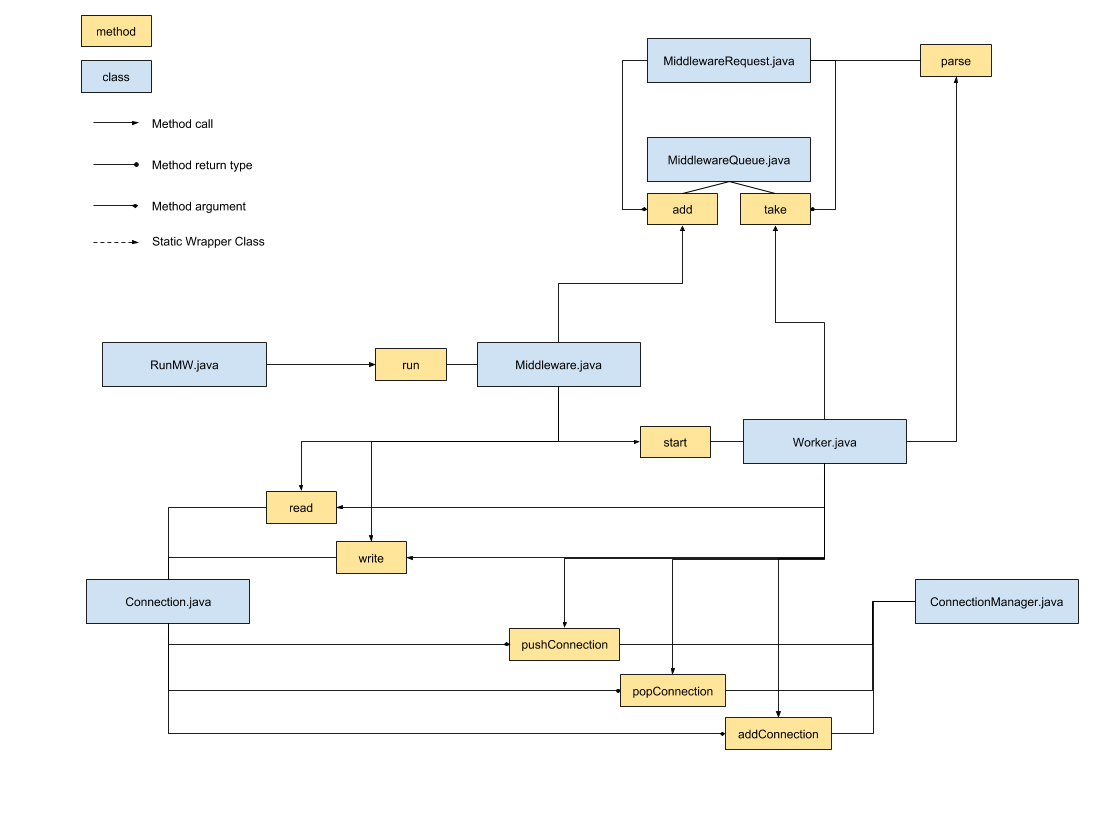
\includegraphics[width=\linewidth]{../illustrations/class_diagram.png}
    \caption{Class Diagram}
    \label{fig:class_diagram}
\end{figure}
%
We will start by looking at a class diagram of the middleware.
%
In Figure~\ref{fig:class_diagram} we can see all the classes that compose the middleware.
%
The system is represented in its running state, i.e. all methods that are only used when starting up are omitted.
%
In the following paragraphs we will look at each of the components in detail.
%
\paragraph{\texttt{RunMW.java}}
%
This class has a single responsibility. It parses the command line arguments and runs the middleware thread using these.
%
\paragraph{\texttt{MiddlewareRequest.java}}
%
This class represents a request coming from a client.
%
The object holds all the relevant data of the request, i.e. all time measurements, whether or not the request was successful and the \texttt{Connection} object of the client that sent the request.
%
In this class we implement the parsing method, that scans the command string and populates fields in the object.
%
If the middleware is running in sharded mode, \texttt{MULTI-GET} requests will be sharded into a list of commands.
%
\paragraph{\texttt{Middleware.java}}
%
This class represents the net thread of the system. Its responsibilities are first to accept client connections and register them so that we can start accepting requests. 
%
Second the thread also reads requests from already acccepted client connections and enqueues them in the \texttt{MiddlewareQueue}.
%
To avoid busy waiting and accessing client sockets that do not have data to read we use a \texttt{Selector}. 
%
Basically this is a mechanism that allows us to register connections and the selector will deliver only the connections that have data ready to read.
%
We also register the server socket with the selector and receive connections that are ready to be accepted.
%
Using this we can maximize the utilization of the CPU time used by the net thread.
%
We will look at the process of accepting connections and requests in detail in section~\ref{subsec:handlingRequests}
%
\paragraph{\texttt{MiddlewareQueue.java}}
%
In this middleware the \texttt{MiddlewareQueue} is a first class citizen, as are the workers and the net thread.
%
This decision is made based on the fact that the queue should not be owned by either the net or the worker threads.
%
The queue is not much more than a static wrapper around a \texttt{BlockingQueue}.
%
The access to take a request out of the queue is synchronized, so that we avoid processing the same request twice.
%
\paragraph{\texttt{Worker.java}}
%
In this class the actual processing of the request is done.
%
Depending on the type of the request that worker threads handle them differently. 
%
This will be adressed in detail in section~\ref{subsec:handlingRequests}.
%
In general a worker thread takes a request out of the \texttt{MiddlewareQueue}, after that the worker calls the parse method offered by \texttt{MiddlewareRequest}.
%
After that several new fields in the request object are populated, such as \texttt{RequestType} for example.
%
The parsed request will then be scheduled on the memcached servers depending on the server mode and request type.
%
The worker then waits for the responses from the memcached servers, parses the responses and then sends the appropriate response to the client.
%
After finishing processing the request the worker will then log the relevant fields for the analysis in a CSV format.
%
\paragraph{\texttt{Connection.java}}
%
The connection class is a convenience wrapper around a \texttt{SocketChannel}.
%
It represents both the client and server connections.
%
It allows us to specify if a connection should be blocking or not.
%
The goal of this class is that when using a connection we do not need to care about the configuration and how to read from the socket, instead we can just call the \texttt{read()} method and the different modes are handled internally.
%
\paragraph{\texttt{ServerManager.java}}
%
This class is used by the worker threads.
%
The \texttt{ServerManager} holds the \texttt{Connection} objects for the memcached servers.
%
This class offers the method \texttt{getConnection(int i)}, which will return the appropriate server connection based on the integer that is passed, such that the load is scheduled in a round robin fashion.
%
We will see in section~\ref{subsec:handlingRequests} how exactly that is handled based on the Id of the request.
%
Even if the request will go to all memcached servers it still makes sense to choose the first server to send the request to based on round robin.
%
This distributes the load even if we only have Set requests.
%
\subsection{Message Parsing}
%
As mentioned before the first thing the workers do with the request is parse it.
%
Parsing means mainly two things here, first we will determine the type of request we are looking at, this tells us how to further handle the request.
%
Second, if applicable, we set the \texttt{MULTI-GET} Size.
%
In the specific case of running the server in sharded mode and receiving a \texttt{MULTI-GET} Request we will split the keys in the request and depending on the \texttt{MULTI-GET} Size and number of servers populate a list of commands, this is known as "sharding" a command.
%
The number of shards is exactly \texttt{min(multiGetSize, numServers)}
%
\subsection{Response Parsing}
%
In two cases, specifically when handling sharded \texttt{MULTI-GET} or \texttt{SET} requests we need to do some work before sending the request to the client.
%
\par
%
In the case of \texttt{SET} requests we need to make sure that the key was set on all the three servers.
%
That can be achieved by simply checking if all the responses equal \texttt{STORED\escape{r}\escape{n}}.
%
If that is the case we send the same response back to the client.
%
If not, it does not matter if we receive an error or if the key was simply not stored on some or all servers, we respond to the client with \texttt{NOT STORED\escape{r}\escape{n}} to let the client know that it should retry setting the key.
%
\par
%
In the case of sharded \texttt{MULTI-GET} requests we need to combine the responses from all servers back to a single response and send it back to the client.
%
This is done by simply removing the end marker from all responses, concatenating them and then adding the end marker back at the end.
%
Finally we count the keys and record how many keys we have received to be able to calculate the miss rate and then we send the response on its way to the client.
%
\subsection{Logs}
%
To handle the logs in this multithreaded setting we use \texttt{log4j}.
%
The logs from all the workers are consolidated into a single CSV file per middleware, this is handled by \texttt{log4j}.
%
After finishing processing a request the workers will call the \texttt{toString()} method implemented by the \texttt{MiddlewareRequest} to produce a CSV log line.
%
This log line is passed to \texttt{log4j}.
%
\subsection{Queues}
%
\begin{figure}[H]
    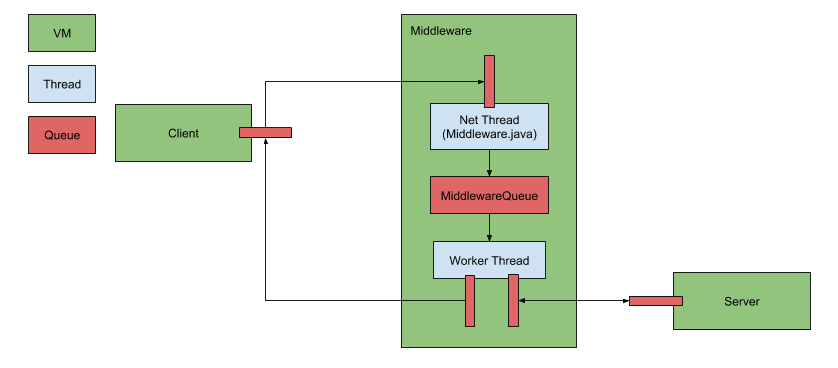
\includegraphics[width=\linewidth]{../illustrations/threads_and_queues.png}
    \caption{Threads and Queues}
    \label{fig:threads_and_queues}
\end{figure}
%
In Figure~\ref{fig:threads_and_queues} we can see an illustration of threads and queues in the system.
%
The arrow directions indicate the flow of requests.
%
Arrows connecting different VMs represent sockets, thus the all queues except the MiddlewareQueue refer to socket queues.
%
The illustration only shows one instance of a client, a server, and a worker thread.
%
In the full system there are three instances of clients and servers.
%
Depending on the configuration there are also many worker threads.
%
The queues and connections for these variable components are also replicated for the number of instances.
%
\subsection{Handling Requests}\label{subsec:handlingRequests}
%
In this section we go into detail on how the middleware handles incoming connections and how the different types of requests are handled by the middleware.
%
What follows are sequence diagrams that model the behaviour of the system for different request types.
%
Important to note here, that again the system is assumed to be in a running state, all the setup methods are executed.
%
Further there are some simplifications and abstractions in the diagrams to reduce clutter, for example not listing all arguments to a method call.
%
Also not all method calls are illustrated, only the ones that are relevant on how we handle different requests.
%
These abstractions should not impact the understanding of the middleware, I tried to design them as self explanatory as possible.
%
Finally the sequence diagrams model the handling of one request, therefore we model only one client and one worker.
%
\begin{figure}[H]
    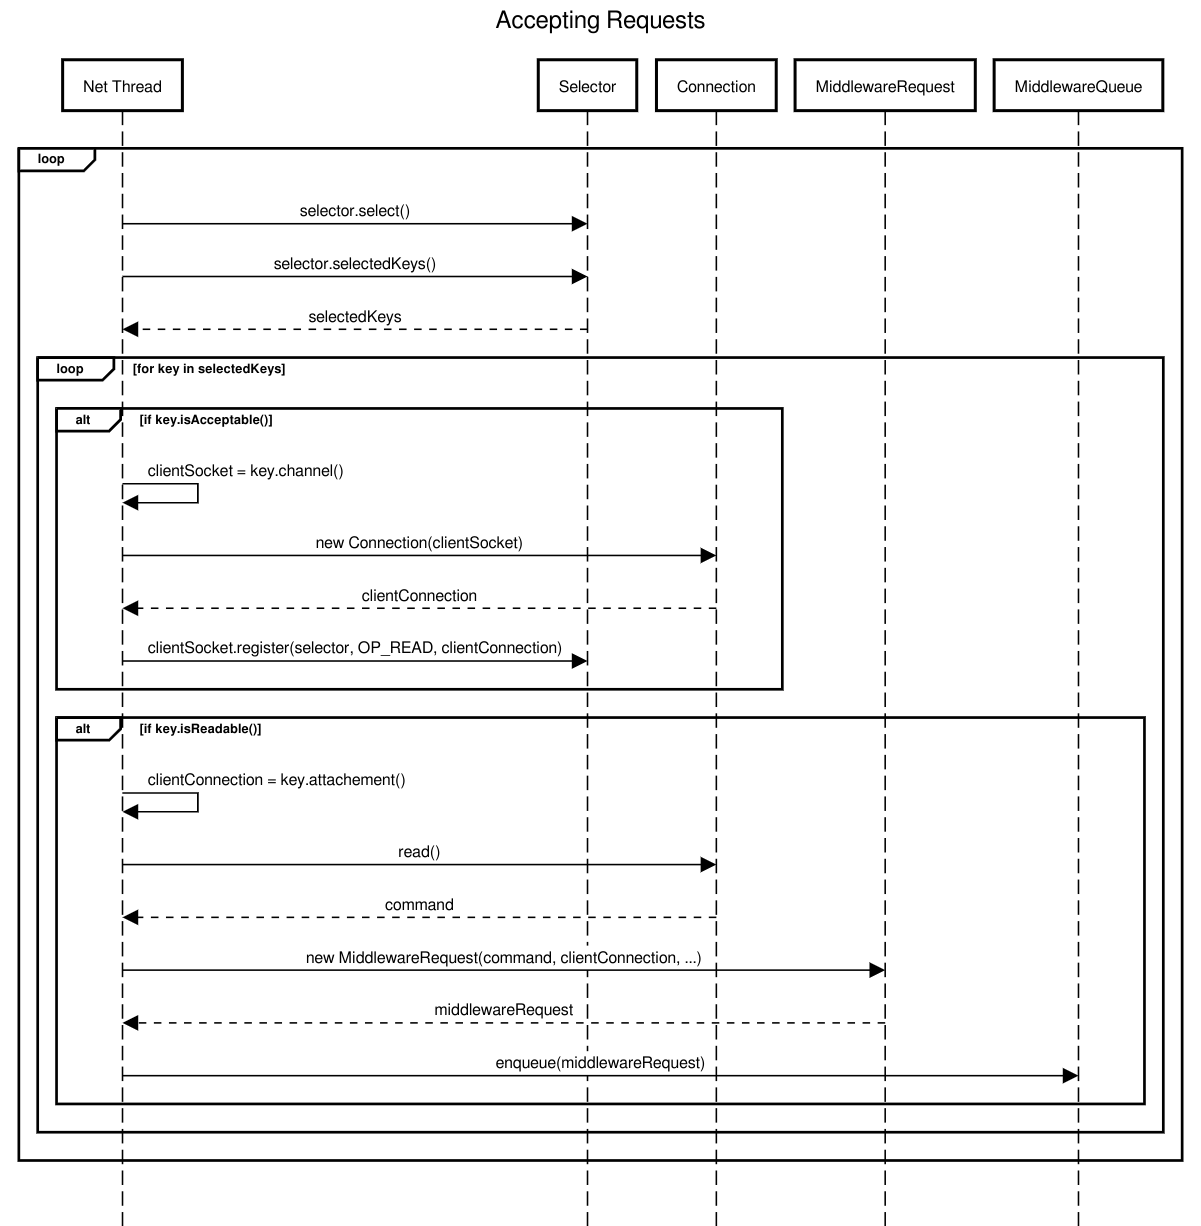
\includegraphics[width=\linewidth]{../illustrations/accepting_requests.png}
    \caption{Accepting new connections and requests}
    \label{fig:accepting_requests}
\end{figure}
%
\begin{figure}[H]
    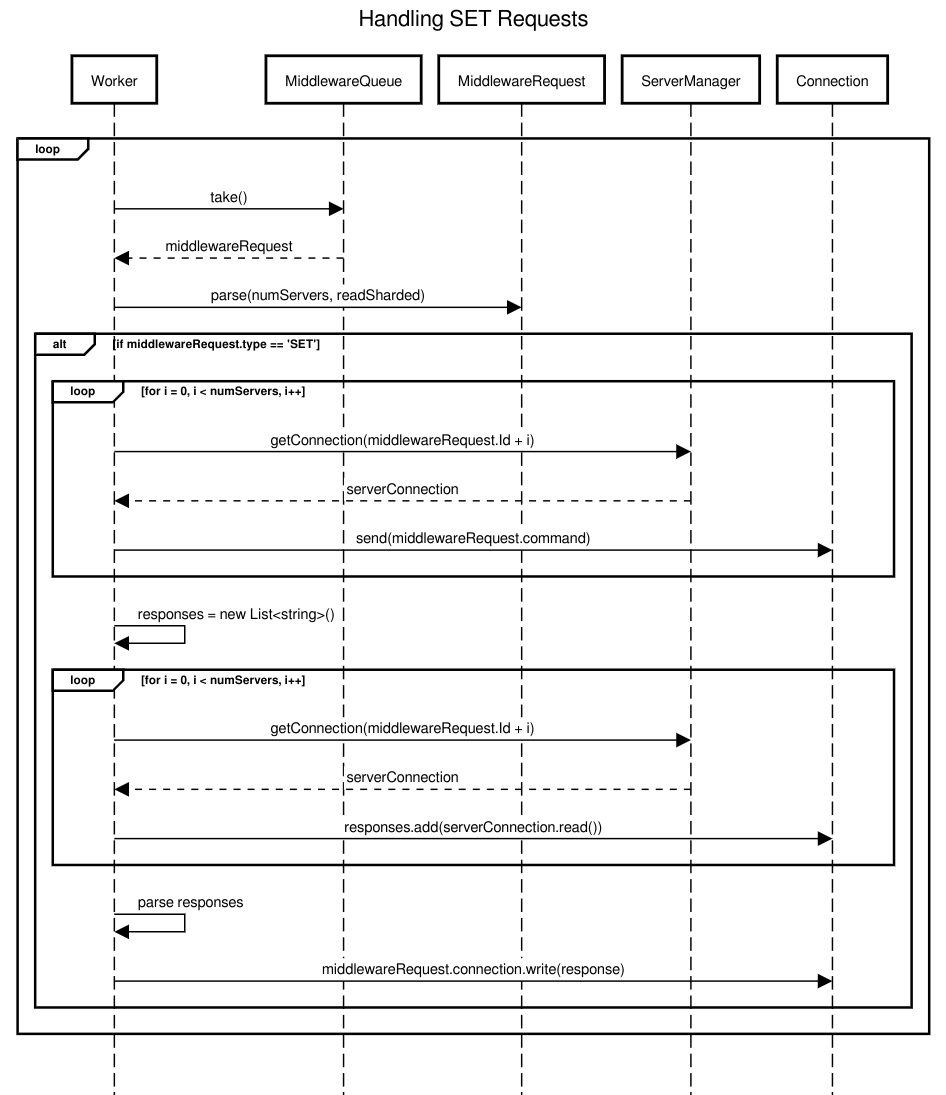
\includegraphics[width=\linewidth]{../illustrations/handling_set.png}
    \caption{Handling \texttt{SET} requests}
    \label{fig:handling_set}
\end{figure}
%
\begin{figure}[H]
    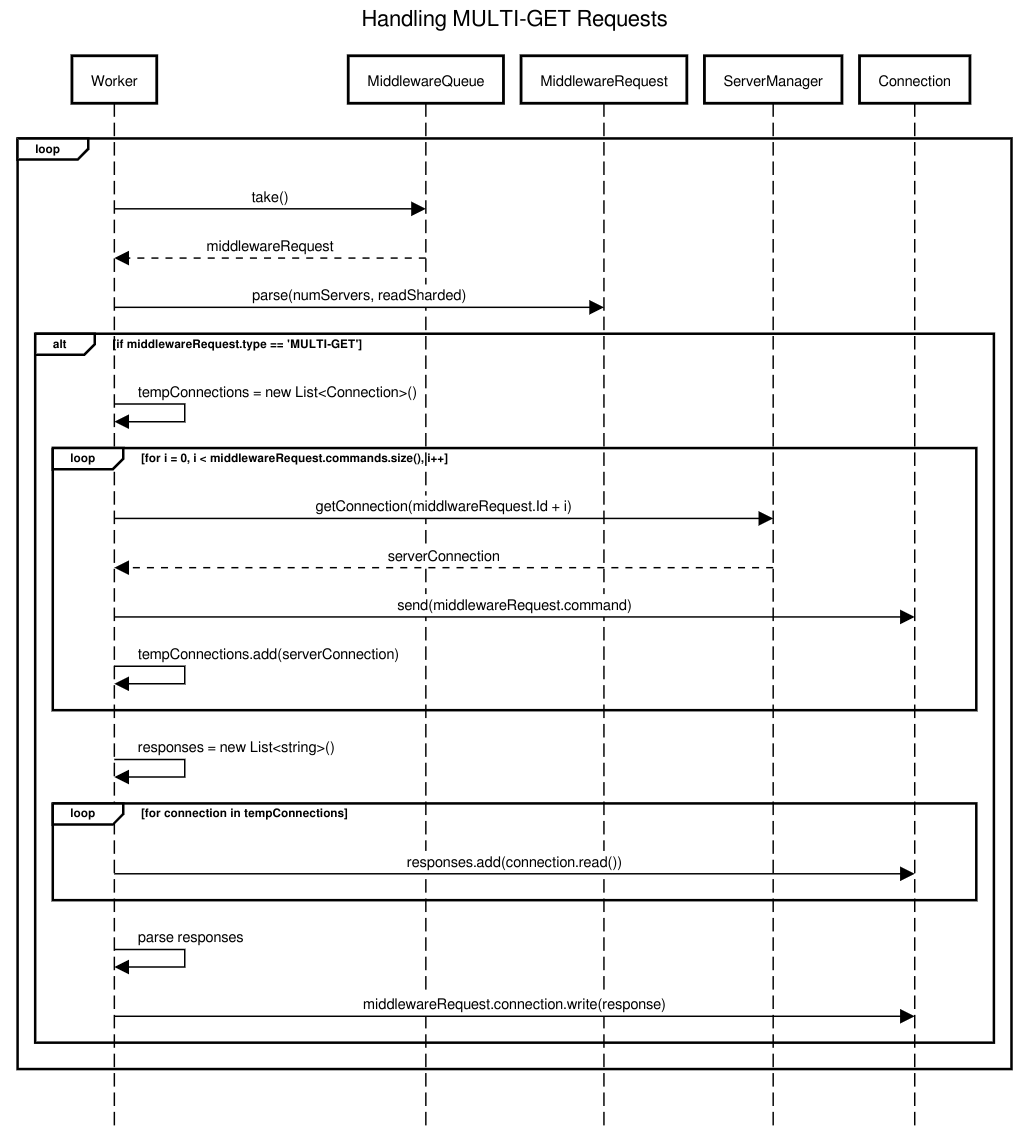
\includegraphics[width=\linewidth]{../illustrations/handling_mget.png}
    \caption{Handling \texttt{MULTI-GET} requests}
    \label{fig:handling_mget}
\end{figure}
%
\begin{figure}[H]
    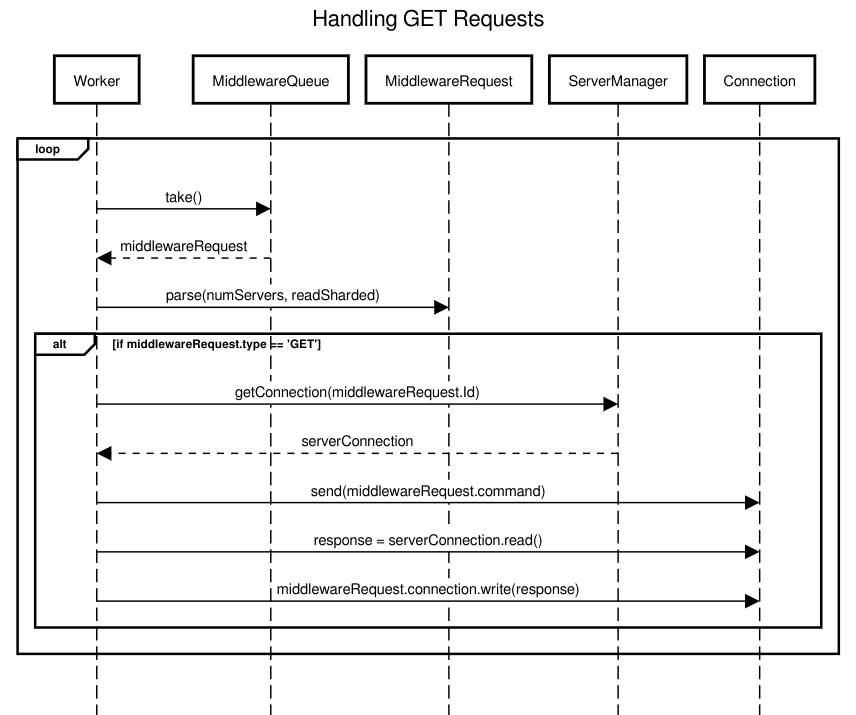
\includegraphics[width=\linewidth]{../illustrations/handling_get.png}
    \caption{Handling \texttt{GET} requests}
    \label{fig:handling_get}
\end{figure}
%
\subsection{Measurements}
%
Before getting into the analysis I want to lose a few words on the measurements and how they are handled.
%
\paragraph{No Middleware}
%
In this case we rely entirely on the output of \texttt{memtier\_benchmark}.
%
There we receive detailed numbers on number of requests and latency, however aggregated per one second intervals.
%
\paragraph{Middleware}
%
In this case we can use the detailed measurements from the middleware logs to produce the plots.
%
The measurements use \texttt{System.nanoTime()} in combination with \\ \texttt{System.currentTimeMillis()} to produce nanosecond Unix Timestamps.
%
We can compute the response time for each request and aggregate the average over all the requests.
%
When computing the average throughput we create a histogram based on the time a request was completed with the same number of bins as the duration of the experiment in seconds.
%
After that we sum these values over all middlewares and compute the average over the seconds the experiments was running.
%
All the plots use the 95\% percent confidence interval as an error measure.
%
\section{Baseline without Middleware (75 pts)}
%
\paragraph{Sanity Checks}
%
In the experiments where we can instrument the middleware we can compute a reasonably good estimate of the think time and therefore produce plots which show that the Interactive Response Time Law holds.
%
In this section however we do not have this information.
%
Here we used pings to get a rough estimate on the think time based on the ping between the machines and used this to manually check if the response time holds for the data in the experiments using one and two memcached servers.
%
\subsection{One Server}
%
\subsubsection{System Setup}
%
For this experiment we will use the following system setup:
%
\begin{itemize}
	\item 3 client machines with 1 memtier instance per machine. Each instance of memtier runs with 2 threads.
	\item No middlewares
	\item 1 memcached server
\end{itemize}
%
We vary the number of virtual clients per thread from 1 to 48.
%
\subsubsection{Hypothesis}
%
The objective of this experiment is to find out how much load a single server can handle.
%
We expect that this can be accomplished since we have 3 load generating machines for one server.
%
\subsubsection{Explanation}\label{sec:one_server_explanantion}
%
\paragraph{Write-Only Workload}
%
\begin{figure}[H]
	\centering
	\captionsetup{width=0.4\textwidth}
    \begin{minipage}{0.5\textwidth}
        \centering
        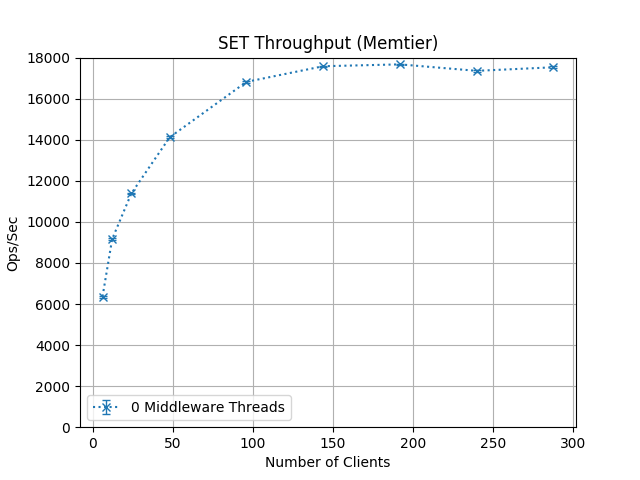
\includegraphics[width=\textwidth]{../illustrations/plots/1_1_one_server/1-0/memtier_set_tp_s.png}
        \caption{\texttt{SET} Throughput}
        \label{fig:one_server_set_tp}
    \end{minipage}\hfill
    \begin{minipage}{0.5\textwidth}
        \centering
        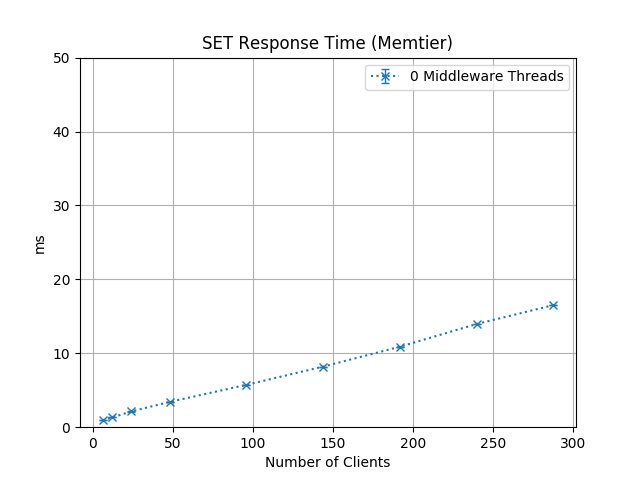
\includegraphics[width=\textwidth]{../illustrations/plots/1_1_one_server/1-0/memtier_set_rt_ms.png}
        \caption{\texttt{SET} Response Time}
        \label{fig:one_server_set_rt}
    \end{minipage}
\end{figure}
%
As mentioned in the objective we want to find out how much, in this case write requests, one memcached server can handle, i.e. how many clients do we need such that the server is saturated.
%
We can see that the server is saturated by two things:
%
\begin{itemize}
	\item The throughput of the system does not increase anymore when increasing the number of clients. We can determine that easily if the throughput plot shows a flat line after some point, however in many cases the throughput does not behave ideally, therefore we need to use other metrics, like the response time, as well to determine saturation.
	\item The response time increases linearly. In an ideal system the response time stays flat when the system is not saturated. However in practice a lot of factors can influence the response time, so it might be increasing in a undersaturated system. What we look for in the response time plot is a "knee" which shows an increase in the amount the response increases per new client. 
\end{itemize}
%
In general we will try to use the two conditions above to determine the point at which the system gets saturated.
%
\par
%
As we can see in Figure~\ref{fig:one_server_set_tp} we can achieve approximately 18000 ops/sec before the server is completely saturated, using 144 clients.
%
However it does not make sense to assume that this throughput can be sustained in a stable way, since according to the throughput we enter the saturation phase already after 96 clients, where adding clients does not increase the throughput significantly anymore.
%
This strategy to determine the point of saturation will be used throughout the experiments, we are interested in what the server can handle in a stable way and not the absolute maximum.
%
In Figure~\ref{fig:one_server_set_rt} it is more difficult to identify the point at which the system is saturated based on the response time, since there is no clear point at which the response time starts to increase.
%
Oversaturation does not occur in this experiment.
%
\par
%
Since this is the very first experiment we cannot yet compare it to much.
%
The take away message here is that one memcached server can handle up to approximately 17000 write ops/sec and is saturated when using 96 clients.
%
Also we conclude definitely that memcached is the bottleneck of the system in this configuration and using this specific workload.
%
\paragraph{Read-Only Workload}
%
\begin{figure}[H]
    \centering
    \captionsetup{width=0.4\textwidth}
    \begin{minipage}{0.5\textwidth}
        \centering
        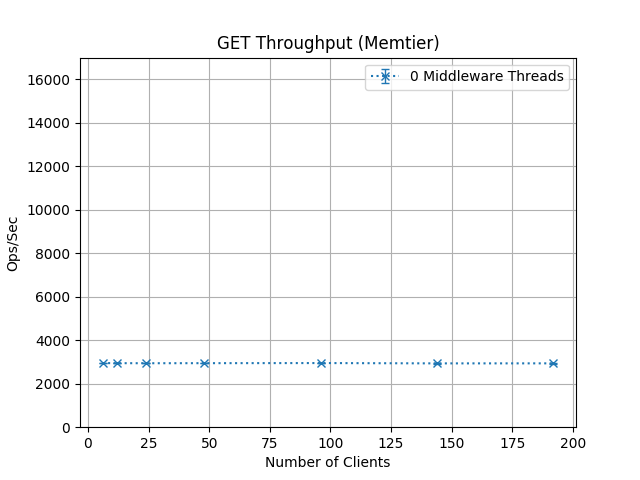
\includegraphics[width=\textwidth]{../illustrations/plots/1_1_one_server/0-1/memtier_get_tp_s.png}
        \caption{\texttt{GET} Throughput}
        \label{fig:one_server_get_tp}
    \end{minipage}\hfill
    \begin{minipage}{0.5\textwidth}
        \centering
        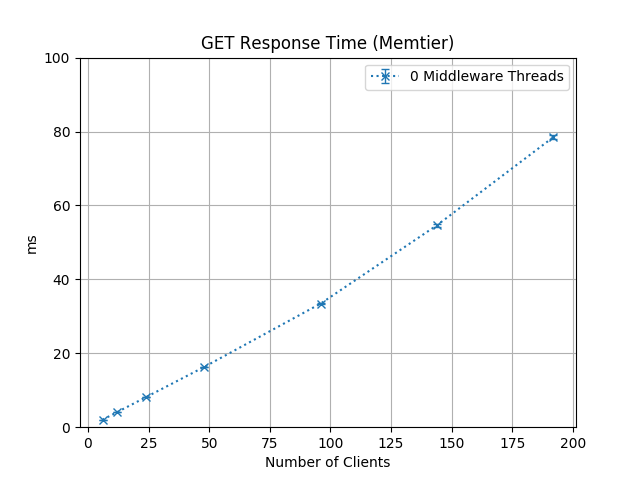
\includegraphics[width=\textwidth]{../illustrations/plots/1_1_one_server/0-1/memtier_get_rt_ms.png}
        \caption{\texttt{GET} Response Time}
        \label{fig:one_server_get_rt}
    \end{minipage}
\end{figure}
%
In Figure~\ref{fig:one_server_get_tp} we see that the system can handle approximately 3000 read ops/sec.
%
As we have seen above the memcached server performs massively better for \texttt{SET} requests.
%
The reason for this is rather straight forward.
%
When handling \texttt{SET} requests the server can just store the record.
%
Usually this is done by hashing the key and storing the value in some sort of hash table, which is a operation that takes $O(1)$ time, since memcached stores all values in memory.
%
However when handling \texttt{GET} requests the server must hash the key, which is still done in constant time, but after hashing the server must actually retrieve the associated value from memory and send it to the client, which takes $O(s)$ time where $s$ is the size of the stored value.
%
The memcached server seems to be saturated even when using only 6 clients.
%
The saturation is clearly depicted in Figure~\ref{fig:one_server_get_tp}, since no matter how many clients we cannot increase the throughput beyond 3000 ops/sec
%
This hypothesis is also supported by the response time, we can see that from the start the response time increases linearly, without increasing the slope at some point during the experiment.
%
Oversaturation does not occur in this experiment even when using 192 virtual clients.
%
\par
%
Since we could not identify an undersaturated phase of the system we ran an additional experiment.
%
The setup was that we used only one load generating machine with only one instance of memtier running only one thread.
%
The virtual clients were varied from 1 to 6, since above we saw an saturation at 6 clients we would expect this experiment to reveal an undersaturated memcached server.
%
\begin{figure}[H]
    \centering
    \captionsetup{width=0.4\textwidth}
    \begin{minipage}{0.5\textwidth}
        \centering
        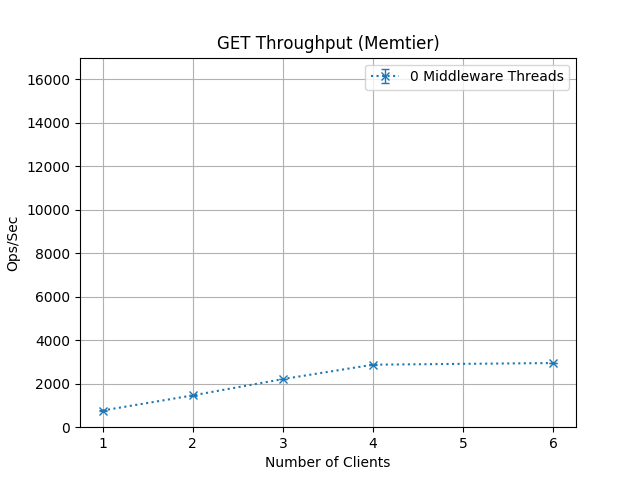
\includegraphics[width=\textwidth]{../illustrations/plots/1_1_1_one_server_reduced/0-1/memtier_get_tp_s.png}
        \caption{\texttt{GET} Throughput}
        \label{fig:one_server_reduced_get_tp}
    \end{minipage}\hfill
    \begin{minipage}{0.5\textwidth}
        \centering
        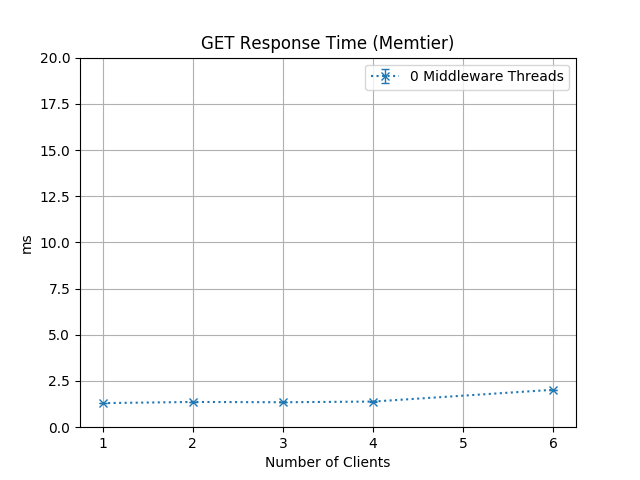
\includegraphics[width=\textwidth]{../illustrations/plots/1_1_1_one_server_reduced/0-1/memtier_get_rt_ms.png}
        \caption{\texttt{GET} Response Time}
        \label{fig:one_server_reduced_get_rt}
    \end{minipage}
\end{figure}
%
As we can see rather clearly in Figure~\ref{fig:one_server_reduced_get_tp} the memcached server is already saturated using only 4 clients in total.
%
\subsection{Two Servers}
%
\subsubsection{System Setup}
%
For this experiment we will use the following system setup:
%
\begin{itemize}
	\item 1 client machines with 2 memtier instances per machine. Each instance of memtier runs with 1 thread.
	\item No middlewares
	\item 2 memcached servers
\end{itemize}
%
We vary the number of virtual clients per thread from 1 to 32.
%
\subsubsection{Hypothesis}
%
Now we have two servers in this experiment and only one load generating machine.
%
Since before the server was the bottleneck in the last experiment we expect the server to be able to handle twice the read load than in the previous experiment.
%
For a write load the server performed very well, and we needed a lot of clients to saturate the servers.
%
In this case we expect memtier to be the bottleneck of the system.
%
\subsubsection{Explanation}
%
\paragraph{Write-Only Workload}
%
\begin{figure}[H]
	\centering
	\captionsetup{width=0.4\textwidth}
    \begin{minipage}{0.5\textwidth}
        \centering
        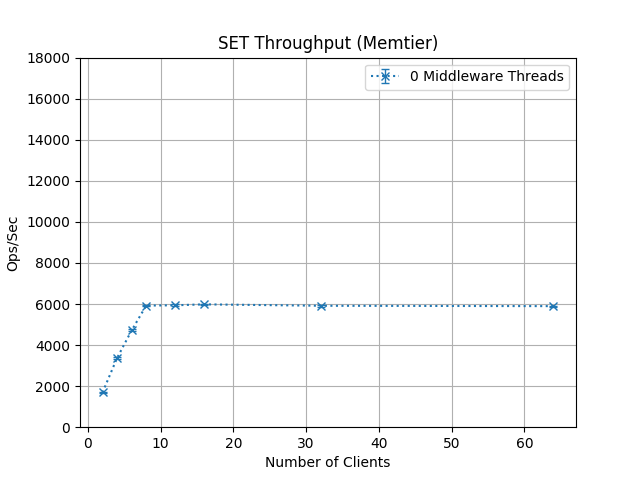
\includegraphics[width=\textwidth]{../illustrations/plots/1_2_two_servers/1-0/memtier_set_tp_s.png}
        \caption{\texttt{SET} Throughput}
        \label{fig:two_servers_set_tp}
    \end{minipage}\hfill
    \begin{minipage}{0.5\textwidth}
        \centering
        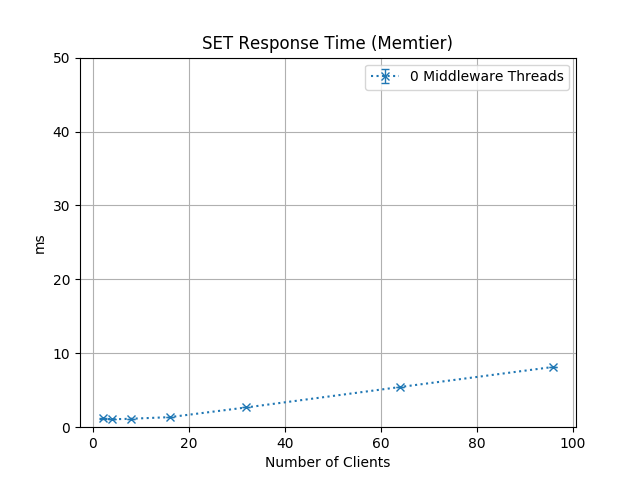
\includegraphics[width=\textwidth]{../illustrations/plots/1_2_two_servers/1-0/memtier_set_rt_ms.png}
        \caption{\texttt{SET} Response Time}
        \label{fig:two_servers_set_rt}
    \end{minipage}
\end{figure}
%
In these two plots we can see both conditions for a saturated phase very clearly.
%
After 16 clients the throughput does not increase at all anymore and reaches a maximum of approximately 6000 write ops/sec.
%
This can be supported by looking at the response time, where we can clearly see the "knee" in the plot after 8 clients.
%
From the previous section we know that one memcached server can handle approximately 17000 write ops/sec which means, since here we have 2 servers, if the servers were the bottleneck we should see double that number.
%
This would lead to the conclusion that the only other participant must be the bottleneck, namely memtier.
%
But in Figure~\ref{fig:two_servers_set_rt} we can see that "knee" in the graph, indicating that the memcached server could be the bottleneck.
%
I still conclude that memtier is the bottleneck, since if we compare the absolute values with Figure~\ref{fig:one_server_set_rt} we quickly see that a saturated memcached server produces response times a lot higher than what we measured in this experiment.
%
It seems as though one client machine cannot produce more than 6000 write ops/sec.
%
\paragraph{Read-Only Workload}
%
\begin{figure}[H]
	\centering
	\captionsetup{width=0.4\textwidth}
    \begin{minipage}{0.5\textwidth}
        \centering
        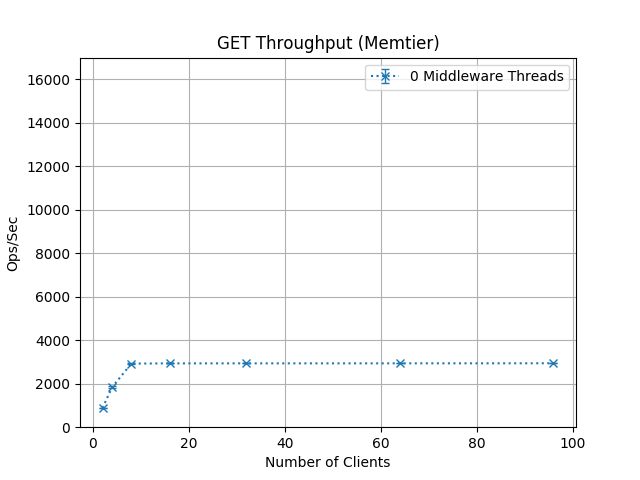
\includegraphics[width=\textwidth]{../illustrations/plots/1_2_two_servers/0-1/memtier_get_tp_s.png}
        \caption{\texttt{GET} Throughput}
        \label{fig:two_servers_get_tp}
    \end{minipage}\hfill
    \begin{minipage}{0.5\textwidth}
        \centering
        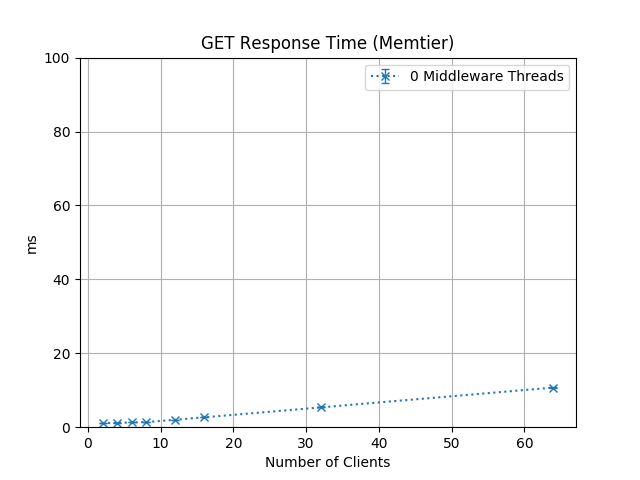
\includegraphics[width=\textwidth]{../illustrations/plots/1_2_two_servers/0-1/memtier_get_rt_ms.png}
        \caption{\texttt{GET} Response Time}
        \label{fig:two_servers_get_rt}
    \end{minipage}
\end{figure}
%
Again here we can clearly the the saturation of the system.
%
However the system is already saturated using only 8 clients in total.
%
This is not surprising since we know from before that \texttt{GET} requests are more expensive for the server than \texttt{SET} requests.
%
What is interesting however is that we can produce almost exactly the same amount of read operations per second than write operations. 
%
From this we conclude that the generation of the payload for \texttt{SET} requests produces a negligible overhead on the client machines.
%
However here it is not as clear cut as before that memtier is the bottleneck.
%
As we saw in Figure~\ref{fig:one_server_get_tp} one server alone can handle approximately 3000 ops/sec, therefore we expect that two saturated memcached servers together can serve about 6000 ops/sec.
%
In Figure~\ref{fig:two_servers_get_tp} we see that in this case we achieve approximately 6000 read ops/sec.
%
This is the exact value we expected from memcached, however it is also the maximum number of requests a client machine can produce.
%
Therefore it is difficult to say exaclty whether memtier or the memcached server are the bottleneck of this system.
%
When we look at Figure~\ref{fig:two_servers_get_rt} we can see that after 8 clients there is an increase in slope, which would indicate that the servers are the bottleneck, since the response time should, in theory, stay constant when the system is undersaturated.
%
Still, there is one argument that paints memtier as the bottleneck.
%
Again we can compare the response time we measure with two servers and compare it to the response time when the memcached server was saturated.
%
The response time in the one server case is a lot higher compared to the response time in this experiment. 
%
This argument lets us conclude fairly certain that memtier must be the bottleneck, since we would measure similar response times as before with saturated server.
%
\subsection{Summary}
%
\begin{center}
	{Maximum throughput of different VMs.}
	\begin{tabular}{|l|p{3cm}|p{3cm}|p{4cm}|}
		\hline                        & Read-only workload & Write-only workload & Configuration gives max. throughput \\ 
		\hline One memcached server   & 2875 (4 Clients)   & 	16818 (96 Clients)  & Write-Only, 96 Clients       \\ 
		\hline One load generating VM & 5810 (8 Clients)  & 5809 (8 Clients)   & Read-Only, 8 Clients         \\ 
		\hline 
	\end{tabular}
\end{center}
%
When we look at the Read-only workload we can see that when we double the amount of servers from one to two the throughput also roughly doubles. 
%
This indicates again that in the first experiment the server is the bottleneck.
%
Further we can see that one server is already saturated with 4 clients, whereas when using two servers we can handle up to 8 clients with approximately double the requests before being saturated, which again supports the conclusion that the server was the bottleneck in the first experiment.
%
\par
%
Looking at the Write-only workload it looks a bit different.
%
We can see that when using less client machines the throughput decreases drastically, even if we use two servers.
%
As mentioned before this indicates that a client machine cannot generate more load.
%
This is because the clients will likely reach their hardware limit at some point, the resources of one machine are shared by too many virtual clients.
%
\par
%
Important to mention is that the numbers above to not always correspond to the absolute maximum throughput observed during the experiments.
%
Instead we will use the throughput that is sustained before the system enters the saturation phase, in the following throughput tables we will do the same thing.
%
\par
%
Summarizing the sections up to now we have a few key take away messages:
%
\begin{itemize}
	\item One memcached server alone can handle a lot more \texttt{SET} requests than \texttt{GET} requests, more than 5 times as much.
	\item One memcached server alone can handle about 17000 \texttt{SET} ops/sec and approximately 3000 \texttt{GET} ops/sec
	\item One client machine alone can generate up to approximately 6000 ops/sec
	\item For one client it does not really matter if it is generating \texttt{GET} or \texttt{SET} requests, when measuring how much ops/sec can be produced.
\end{itemize}
%
The absolute numbers here should only be used as an approximate measure, even just restarting the VMs can produce different results. 
%
\section{Baseline with Middleware (90 pts)}
%
\subsection{One Middleware}
%
\subsubsection{System Setup}
%
For this experiment we will use the following system setup:
%
\begin{itemize}
	\item 3 client machines with 1 memtier instances per machine. Each instance of memtier runs with 2 threads.
	\item 1 middleware
	\item 1 memcached server
\end{itemize}
%
We vary the number of virtual clients per thread from 1 to 40.
%
\subsubsection{Hypothesis}
%
Similar to the first experiment we will find out how much load a single middleware can handle
%
We assume for now that one memcached server is more performing than the middleware and therefore it should not be a problem that we only use one server.
%
We will see later if this assumption is justified.
%
In this experiment we only use one server, therefore the middleware should not generate any overhead for synchronizing \texttt{SET} requests across multiple servers.
%
Therefore we expect also in this case that \texttt{SET} requests will have a higher throughput than \texttt{GET} requests.
%
Also as we increase the number of worker threads, more clients should be needed to saturate the system.
%
\subsubsection{Explanation}\label{subsec:one_middleware_explanation}
%
\paragraph{Write-Only Workload}
%
\begin{figure}[H]
	\centering
	\captionsetup{width=0.4\textwidth}
    \begin{minipage}{0.5\textwidth}
        \centering
        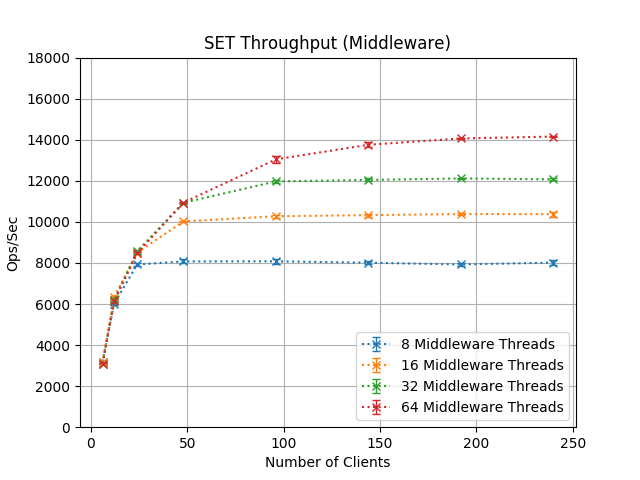
\includegraphics[width=\textwidth]{../illustrations/plots/2_1_one_middleware/1-0/middleware_set_tp_s.png}
        \caption{\texttt{SET} Throughput}
        \label{fig:one_middleware_set_tp_mw}
    \end{minipage}\hfill
    \begin{minipage}{0.5\textwidth}
        \centering
        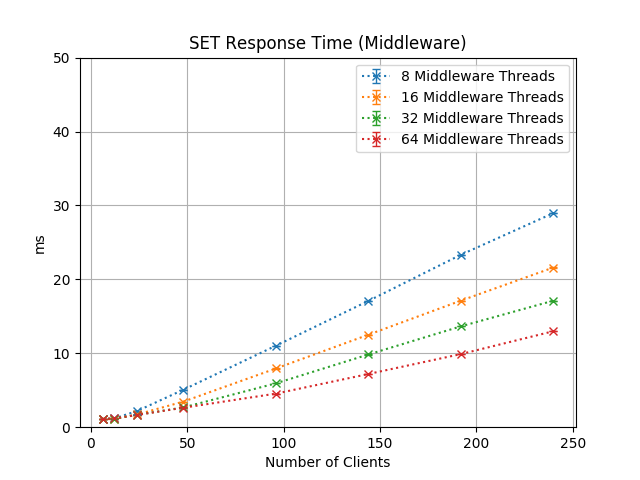
\includegraphics[width=\textwidth]{../illustrations/plots/2_1_one_middleware/1-0/middleware_set_rt_ms.png}
        \caption{\texttt{SET} Response Time}
        \label{fig:one_middleware_set_rt_mw}
    \end{minipage}
\end{figure}
%
\begin{figure}[H]
	\centering
	\captionsetup{width=0.4\textwidth}
    \begin{minipage}{0.5\textwidth}
        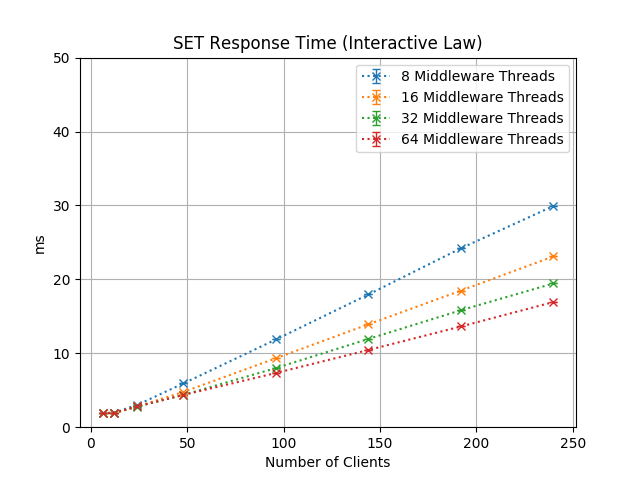
\includegraphics[width=\textwidth]{../illustrations/plots/2_1_one_middleware/1-0/middleware_interactive_set_rt_ms.png}
        \caption{\texttt{SET} Response time IRTL}
        \label{fig:one_middleware_set_rt_it}
    \end{minipage}\hfill
\end{figure}
%
\begin{figure}[H]
	\centering
	\captionsetup{width=0.4\textwidth}
    \begin{minipage}{0.5\textwidth}
        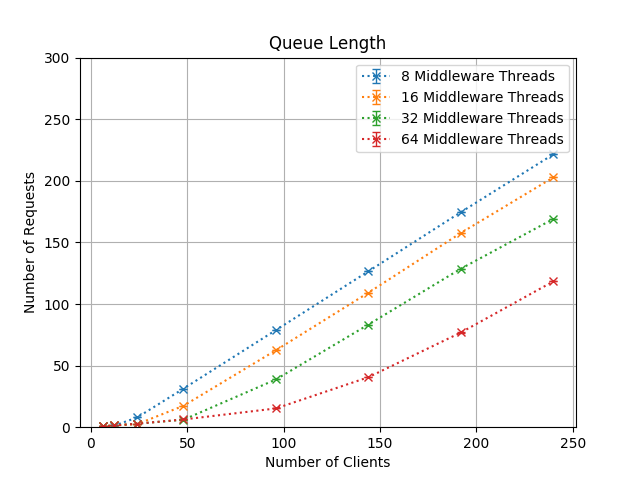
\includegraphics[width=\textwidth]{../illustrations/plots/2_1_one_middleware/1-0/middleware_queue_length.png}
        \caption{\texttt{SET} Queue Length}
        \label{fig:one_middleware_set_ql}
    \end{minipage}\hfill
    \begin{minipage}{0.5\textwidth}
        \centering
        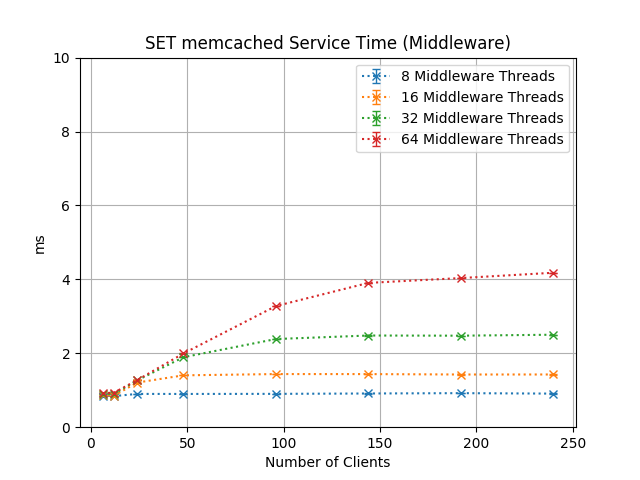
\includegraphics[width=\textwidth]{../illustrations/plots/2_1_one_middleware/1-0/middleware_set_service_time_ms.png}
        \caption{\texttt{SET} Service Time of memcached}
        \label{fig:one_middleware_set_st_mw}
    \end{minipage}
\end{figure}
%
Before discussing the system I quickly want to mention Figure~\ref{fig:one_middleware_set_rt_it}, throughout the report we will find these plots for all experiments.
%
The Interactive Response Time Law gives us a relationship between the throughput and the response time of the system. The exact formula is:
%
\[
R = \left(\frac{N}{X}\right) - Z
\]
%
Where $R$ is the response time, $X$ the throughput, $N$ the number of clients and finally $Z$ is the so called think time.
%
It is the time a client needs to produce another request.
%
Using the data collected inside the middleware we can estimate this time, by looking at how long it takes after a worker has responsed to the client until a new request from the same client is received in the net thread.
%
However since analyzing this is extremely time consuming, since for each combination of client, worker and middleware we need to sort the values and compute this time, we estimated this using the time a woker is idle.
%
To motivate this we looked at a sample where we checked the difference between the two numbers, and since the difference between the two is constant and small, which means the net thread and network latency do not add significant overhead, it is reasonable to take this as an estimation for the think time.
%
\par
%
The rest of the variables are measured by the middleware as well.
%
Now we can estimate the response time based on the throughput, think time and the number of clients.
%
These plots should serve as a sanity check for the measurements.
%
However since the think time is estimated, also the resulting response time will be an estimation on the real response time.
%
As long as the response time from the interactive law and the measured response time behave similarly, we can assume that the response time and throughput measured is realistic.
%
In the following experiments I will include this plot, but I will not mention it every time.
%
\par
%
Now if we look at Figure~\ref{fig:one_middleware_set_tp_mw} we can see that the system enters the saturation phase when using more than 12 clients with 8 threads, 24 clients with 16 threads, 48 clients using 32 threads and 96 clients with 64 worker threads.
%
The same can be seen in Figure~\ref{fig:one_middleware_set_rt_mw}, although not that clearly, where the response time starts to increase at the same thresholds.
%
To motivate the choice of saturation thresholds more we can look at Figure~\ref{fig:one_middleware_set_ql}.
%
We can see that the queue length starts to increase at the same threshold levels.
%
This indicates that the system is saturated, i.e. that requests will be waiting in the queue after these points.
%
Of course the thresholds are not exact numbers, since we would need to run the experiment for all possible number of clients, however we are interested in what we can assume the server can handle in a stable fashion, therefore we choose the thresholds as above.
%
As we can further see in Figure~\ref{fig:one_middleware_set_tp_mw} the maximum throughput we can achieve is approximately 13000 ops/sec.
%
From the experiments using only one server we know however that one memcached server can handle up to approx. 17000 ops/sec.
%
This would indicate that the middleware is the bottleneck in all worker thread configurations in this experiment.
%
This conclusion can be supported by Figure~\ref{fig:one_middleware_set_st_mw} where we can see that the service time of the servers does not increase beyond 4 msecs, which strongly suggests the memcached server is undersaturated.
%
Therefore we can conclude here that the middleware is the bottleneck, and that the middleware can handle up to 13000 \texttt{SET} ops/sec, as long as the middleware does not need to coordinate those requests across multiple servers.
%
Oversaturation did not occur in this experiment.
%
\paragraph{Read-Only Workload}
%
\begin{figure}[H]
	\centering
	\captionsetup{width=0.4\textwidth}
    \begin{minipage}{0.5\textwidth}
        \centering
        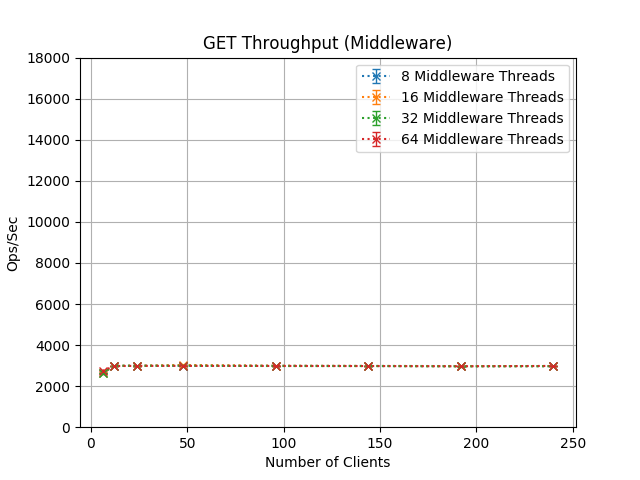
\includegraphics[width=\textwidth]{../illustrations/plots/2_1_one_middleware/0-1/middleware_get_tp_s.png}
        \caption{\texttt{GET} Throughput}
        \label{fig:one_middleware_get_tp_mw}
    \end{minipage}\hfill
    \begin{minipage}{0.5\textwidth}
        \centering
        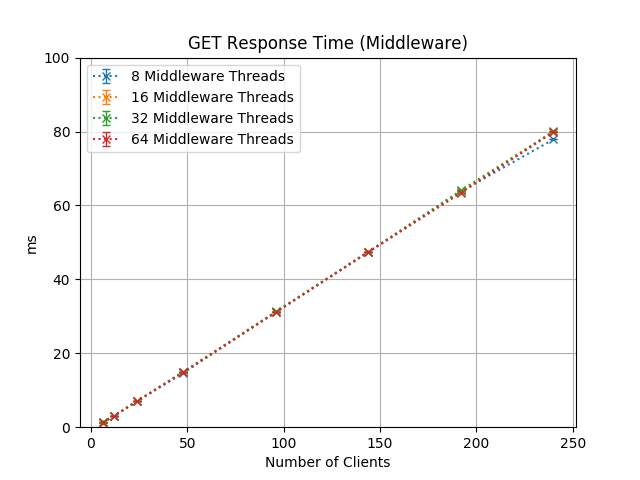
\includegraphics[width=\textwidth]{../illustrations/plots/2_1_one_middleware/0-1/middleware_get_rt_ms.png}
        \caption{\texttt{GET} Response Time}
        \label{fig:one_middleware_get_rt_mw}
    \end{minipage}
\end{figure}
%
\begin{figure}[H]
	\centering
	\captionsetup{width=0.4\textwidth}
    \begin{minipage}{0.5\textwidth}
        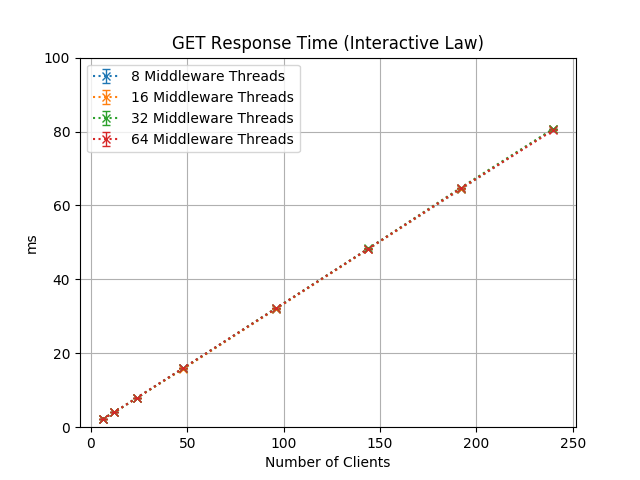
\includegraphics[width=\textwidth]{../illustrations/plots/2_1_one_middleware/0-1/middleware_interactive_get_rt_ms.png}
        \caption{\texttt{GET} Response time according to Interactive Law based on Throughput}
        \label{fig:one_middleware_get_rt_it}
    \end{minipage}\hfill
\end{figure}
%
\begin{figure}[H]
	\centering
	\captionsetup{width=0.4\textwidth}
    \begin{minipage}{0.5\textwidth}
        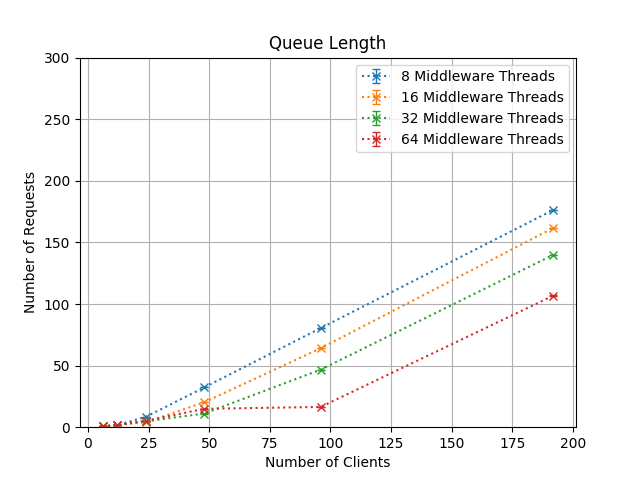
\includegraphics[width=\textwidth]{../illustrations/plots/2_1_one_middleware/0-1/middleware_queue_length.png}
        \caption{\texttt{GET} Queue Length}
        \label{fig:one_middleware_get_ql}
    \end{minipage}\hfill
    \begin{minipage}{0.5\textwidth}
        \centering
        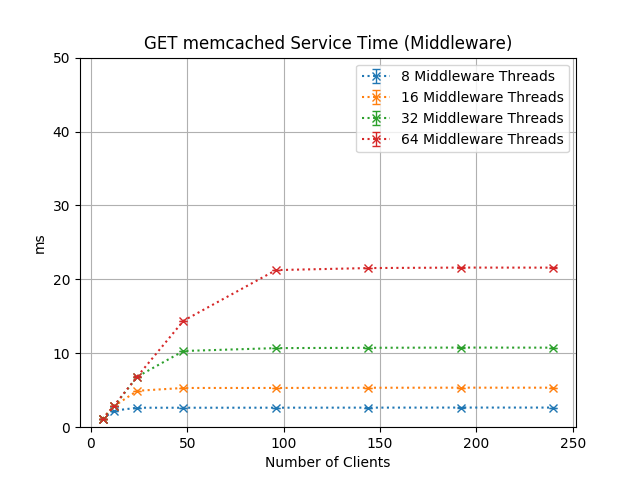
\includegraphics[width=\textwidth]{../illustrations/plots/2_1_one_middleware/0-1/middleware_get_service_time_ms.png}
        \caption{\texttt{GET} Service Time of memcached}
        \label{fig:one_middleware_get_st_mw}
    \end{minipage}
\end{figure}
%
In the first experiments we learned that one memcached server can handle up to 3000 ops/sec.
%
Here we see this value again in Figure~\ref{fig:one_middleware_get_tp_mw}, therefore we suspect that the memcached server is the bottleneck.
%
The response time also behaves similarly as in the experiment using only one server.
%
But in this case we can again look at Figure~\ref{fig:one_middleware_get_st_mw} and see how the service time for the memcached server behaves.
%
We can quickly see that at first it is correct that memcached is the bottleneck, since the service time increases linearly with the number of clients.
%
However at some point the service time stays flat.
%
Specifically at 24 clients using 8 threads, at 48 clients for 16 and 32 threads, and finally at 96 clients for 64 threads.
%
At first glance it seems that the middleware is the bottleneck since the service time of the servers does not increase anymore.
%
\par
%
What happens inside the middleware, is that each of the workers is processing a request at all times. 
%
For the memcached server that means that it sees only 64 clients, which are behaving similarly to the memtier clients, namely sending a request as soon as the previous request is completed.
%
Again we can use support this conclusion by looking at Figure~\ref{fig:one_middleware_get_ql} where we see the queue length increase at the same point where the service time of memcached does not increase anymore, showing that the worker threads cannot handle more requests.
%
But here it is important to compare this to the first experiment where we only used one server.
%
In Figure~\ref{fig:one_server_get_rt} we can see that we have a similar response time as we do now, meaning the middleware does not add any significant overhead.
%
The middleware starts buffering requests from clients, but the bottleneck is still the server.
%
Since in this case we handle \texttt{GET} requests exactly the same as we would handle \texttt{SET} requests we can say with confidence that the middleware would process these requests at the same rate, which is a lot higher than what we are seeing in this experiment.
%
Using these arguments we conclude that, here too the server is the bottleneck of the system.
%
Again oversaturation did not occur.
%
\par
%
Also in this experiment we could not really see the system in a undersaturated phase.
%
For that we ran another experiment with the same configuration as in section~\ref{sec:one_server_explanantion}.
%
\begin{figure}[H]
	\centering
	\captionsetup{width=0.4\textwidth}
    \begin{minipage}{0.5\textwidth}
        \centering
        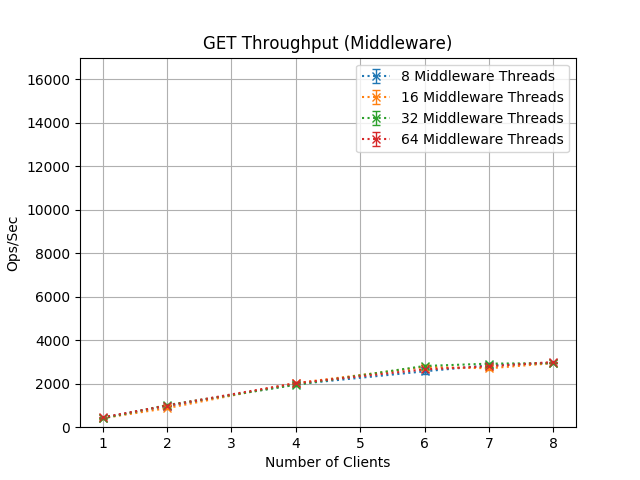
\includegraphics[width=\textwidth]{../illustrations/plots/2_1_1_one_middleware_reduced/0-1/middleware_get_tp_s.png}
        \caption{\texttt{GET} Throughput}
        \label{fig:one_middleware_reduced_get_tp_mw}
    \end{minipage}\hfill
    \begin{minipage}{0.5\textwidth}
        \centering
        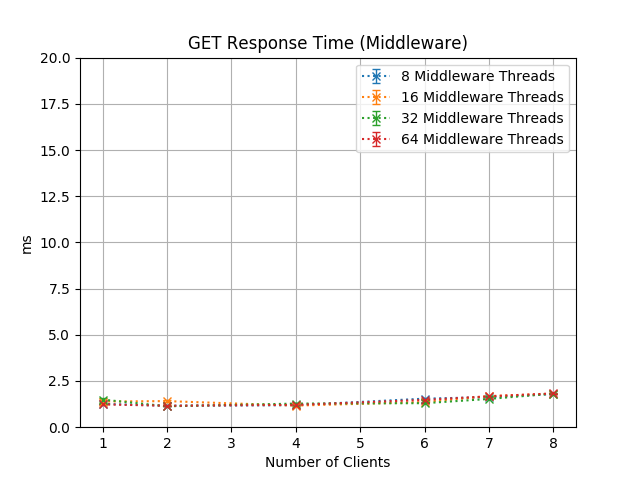
\includegraphics[width=\textwidth]{../illustrations/plots/2_1_1_one_middleware_reduced/0-1/middleware_get_rt_ms.png}
        \caption{\texttt{GET} Response Time}
        \label{fig:one_middleware_reduced_get_rt_mw}
    \end{minipage}
\end{figure}
%
As we can see, we can saturate the system using \texttt{GET} requests already at 6 total clients.
%
In Figure~\ref{fig:one_middleware_reduced_get_rt_mw} we can see a few anomalies when using one and two clients, however in combination with Figure~\ref{fig:one_middleware_reduced_get_tp_mw} we can find slight increase in the response time at 6 clients.
%
Of course these numbers are rather small, therefore it is not as clear as in the above illustrations, however the goal is to show the system in an undersaturated state, which these plots certainly do.
%
\subsection{Two Middlewares}
%
\subsubsection{System Setup}
%
For this experiment we will use the following system setup:
%
\begin{itemize}
	\item 3 client machines with 2 memtier instances per machine. Each instance of memtier runs with 1 threads.
	\item 2 middlewares
	\item 1 memcached server
\end{itemize}
%
We vary the number of virtual clients per thread from 1 to 40, except for the 64 threads configuration where we added a datapoint at 48 clients.
%
This was done to show that the datapoint at 240 clients is a bit of an outlier and we wanted to be sure that the throughput does not increase even more.
%
\subsubsection{Hypothesis}
%
We expect this configuration to handle twice the load as with one middleware before becoming saturated, assuming the server will not bottleneck the system.
%
Again we only use one server, therefore we expect again in this case that \texttt{SET} requests will have a higher throughput than \texttt{GET} requests.
%
Further as we increase the number of worker threads, more clients should be needed to saturate the system.
%
\subsubsection{Explanation}\label{subsec:two_middlewares_explanation}
%
\paragraph{Write-Only Workload}
%
\begin{figure}[H]
	\centering
	\captionsetup{width=0.4\textwidth}
    \begin{minipage}{0.5\textwidth}
        \centering
        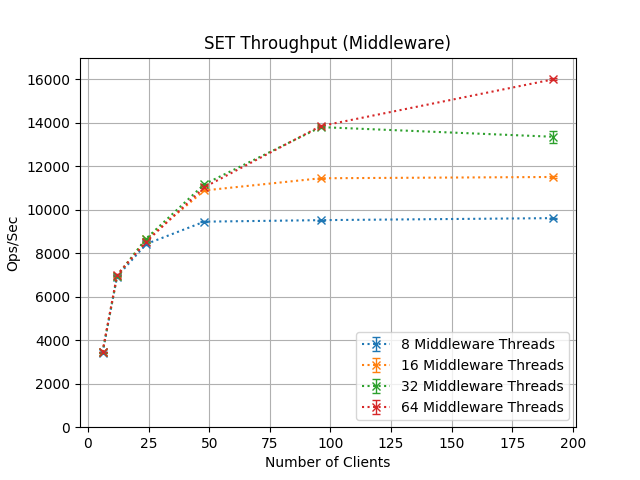
\includegraphics[width=\textwidth]{../illustrations/plots/2_2_two_middlewares/1-0/middleware_set_tp_s.png}
        \caption{\texttt{SET} Throughput}
        \label{fig:two_middlewares_set_tp_mw}
    \end{minipage}\hfill
    \begin{minipage}{0.5\textwidth}
        \centering
        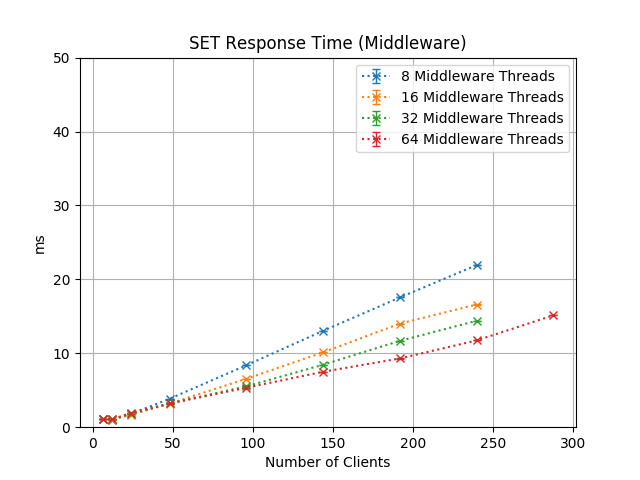
\includegraphics[width=\textwidth]{../illustrations/plots/2_2_two_middlewares/1-0/middleware_set_rt_ms.png}
        \caption{\texttt{SET} Response Time}
        \label{fig:two_middlewares_set_rt_mw}
    \end{minipage}
\end{figure}
%
\begin{figure}[H]
	\centering
	\captionsetup{width=0.4\textwidth}
    \begin{minipage}{0.5\textwidth}
        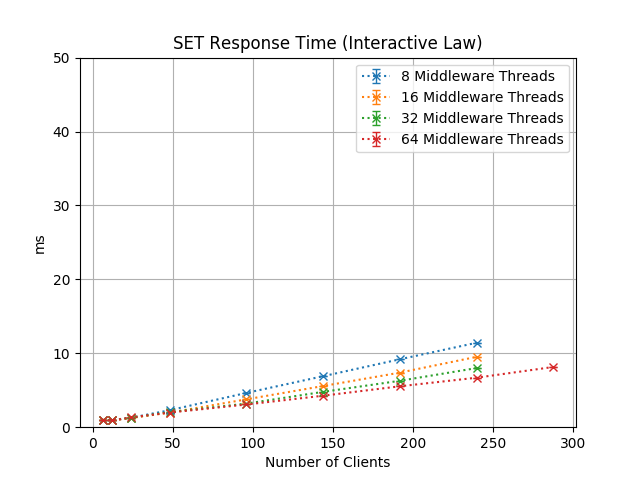
\includegraphics[width=\textwidth]{../illustrations/plots/2_2_two_middlewares/1-0/middleware_interactive_set_rt_ms.png}
        \caption{\texttt{SET} Response time IRTL}
        \label{fig:two_middlewares_set_rt_it}
    \end{minipage}\hfill
\end{figure}
%
\begin{figure}[H]
	\centering
	\captionsetup{width=0.4\textwidth}
    \begin{minipage}{0.5\textwidth}
        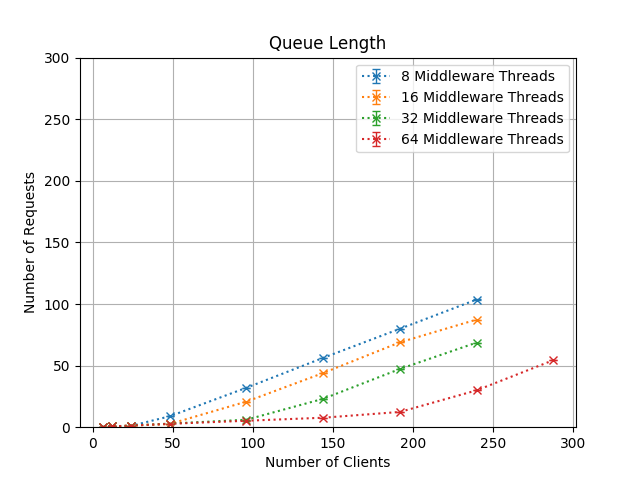
\includegraphics[width=\textwidth]{../illustrations/plots/2_2_two_middlewares/1-0/middleware_queue_length.png}
        \caption{\texttt{SET} Queue Length}
        \label{fig:two_middlewares_set_ql}
    \end{minipage}\hfill
    \begin{minipage}{0.5\textwidth}
        \centering
        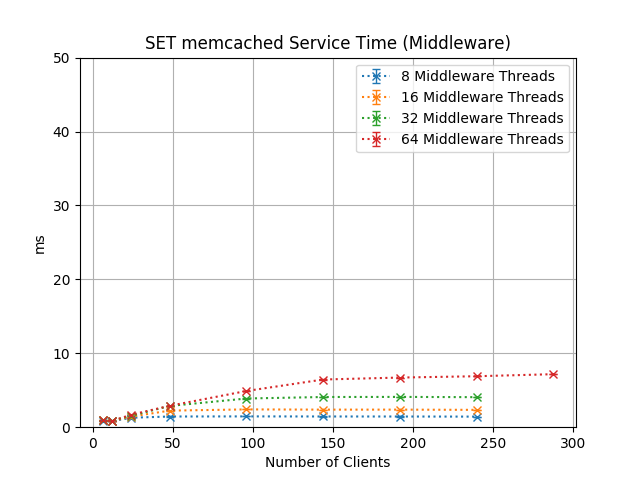
\includegraphics[width=\textwidth]{../illustrations/plots/2_2_two_middlewares/1-0/middleware_set_service_time_ms.png}
        \caption{\texttt{SET} Service Time of memcached}
        \label{fig:two_middlewares_set_st_mw}
    \end{minipage}
\end{figure}
%
By looking at Figure~\ref{fig:two_middlewares_set_tp_mw} we see that we can handle approximately 24 clients for 8 threads, 48 clients for 16 threads, 96 clients for 32 threads and finally 192 clients for 64 threads before the system is saturated.
%
From section~\ref{sec:one_server_explanantion} we know that one server can handle approximately 17000 write ops/sec, before being saturated.
%
As we can see in Figure~\ref{fig:two_middlewares_set_tp_mw} in this experiment we achieve approximately the same number when using two middlewares with 64 threads and one server, but for all other configurations we are significantly below that.
%
This is a first indication that for the three smaller configurations the middlewares are the bottleneck.
%
\par
%
We can confirm the assumption that the middlewares are the bottleneck by looking at Figure~\ref{fig:two_middlewares_set_st_mw} which shows that for 8, 16 and 32 threads the service time of memcached stays almost constant, indicating that the server is not saturated. 
%
Even though the server is not saturated and the service time is only almost constant, the response time still increases.
%
That means that in these cases the middleware must be the bottleneck, since we have 3 load generating machines, which are able to produce plenty of requests to saturate the memcached server.
%
We can further support this conclusion by looking at the queue length in the middleware, there we can see at the same threshold the requests begin to wait in the queue indicating that the above conclusion is sound.
%
\par
%
However the configuration using 64 threads is a bit more difficult.
%
First we can see that when the system is saturated we can handle approximately 17000 ops/sec which, as mentioned before, should saturate the server.
%
However when looking at Figure~\ref{fig:two_middlewares_get_st_mw} we do not observe a linear increase in service time after using 192 clients.
%
But again we need to be aware that in principle the middlewares simulate, in this case, 128 clients to the memcached server.
%
Thus we must compare the performance of one server using 128 clients with the performance here, since all the workers are processing requests all the time.
%
Using a similar argumentation as for \texttt{GET} requests in the previous experiment we can compare the service time of memcached to the response time using approximately 128 in Figure~\ref{fig:one_server_set_rt}.
%
We can immediately see that the memcached server behaves almost the same in terms of response time and throughput as when did not use any middleware.
%
Further we saw in the one server experiment that the memcached server is saturated after using 96 clients.
%
Putting the above arguments together we can conclude that when using 64 clients we can saturate the memcached server using 2 middlewares.
%
\paragraph{Read-Only Workload}
%
\begin{figure}[H]
	\centering
	\captionsetup{width=0.4\textwidth}
    \begin{minipage}{0.5\textwidth}
        \centering
        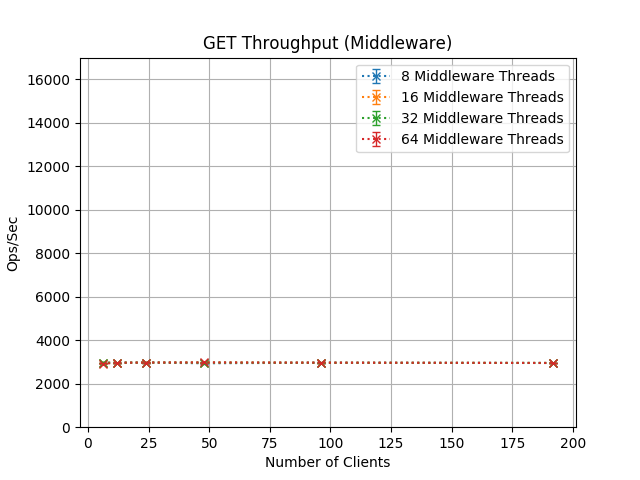
\includegraphics[width=\textwidth]{../illustrations/plots/2_2_two_middlewares/0-1/middleware_get_tp_s.png}
        \caption{\texttt{GET} Throughput}
        \label{fig:two_middlewares_get_tp_mw}
    \end{minipage}\hfill
    \begin{minipage}{0.5\textwidth}
        \centering
        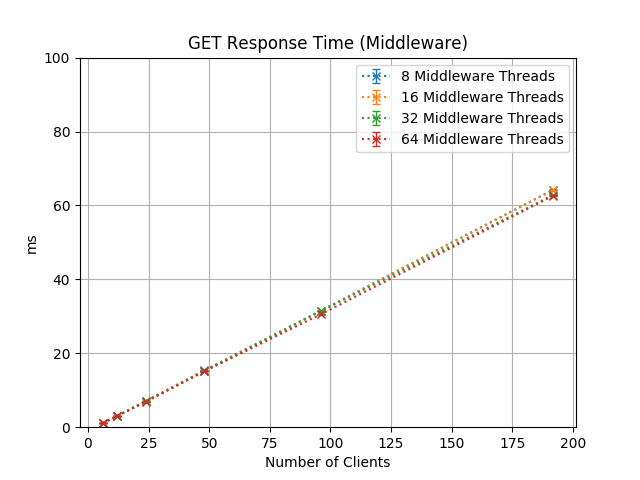
\includegraphics[width=\textwidth]{../illustrations/plots/2_2_two_middlewares/0-1/middleware_get_rt_ms.png}
        \caption{\texttt{GET} Response Time}
        \label{fig:two_middlewares_get_rt_mw}
    \end{minipage}
\end{figure}
%
\begin{figure}[H]
	\centering
	\captionsetup{width=0.4\textwidth}
    \begin{minipage}{0.5\textwidth}
        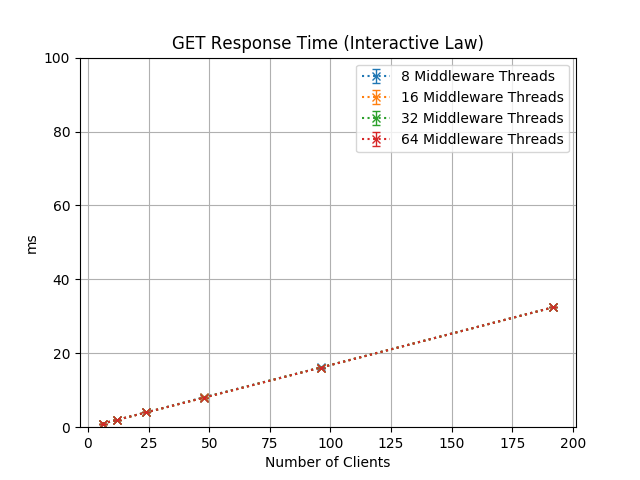
\includegraphics[width=\textwidth]{../illustrations/plots/2_2_two_middlewares/0-1/middleware_interactive_get_rt_ms.png}
        \caption{\texttt{GET} Response time according to Interactive Law based on Throughput}
        \label{fig:two_middlewares_get_rt_it}
    \end{minipage}\hfill
\end{figure}
%
\begin{figure}[H]
	\centering
	\captionsetup{width=0.4\textwidth}
    \begin{minipage}{0.5\textwidth}
        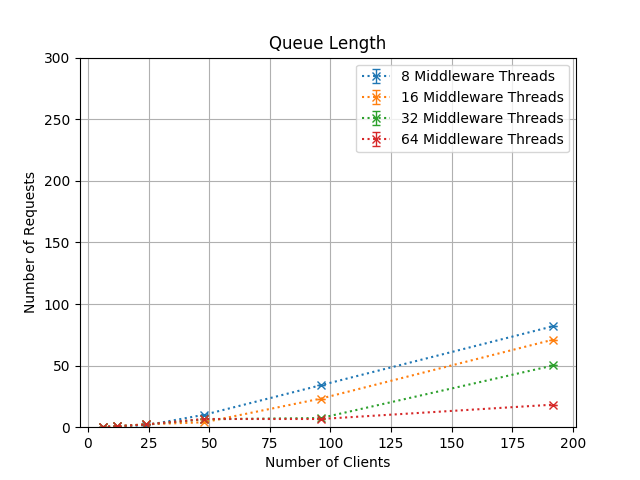
\includegraphics[width=\textwidth]{../illustrations/plots/2_2_two_middlewares/0-1/middleware_queue_length.png}
        \caption{\texttt{GET} Queue Length}
        \label{fig:two_middlewares_get_ql}
    \end{minipage}\hfill
    \begin{minipage}{0.5\textwidth}
        \centering
        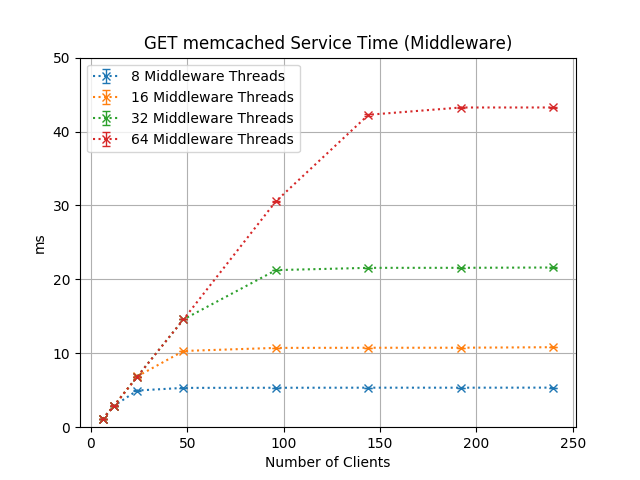
\includegraphics[width=\textwidth]{../illustrations/plots/2_2_two_middlewares/0-1/middleware_get_service_time_ms.png}
        \caption{\texttt{GET} Service Time of memcached}
        \label{fig:two_middlewares_get_st_mw}
    \end{minipage}
\end{figure}
Again we use only one server here, so we expect the system to be saturated again at approximately 3000 ops/sec.
%
We can verify this in Figure~\ref{fig:two_middlewares_get_tp_mw}.
%
As usual by looking at the throughput plot using one server we cannot really identify the bottleneck, since it is saturated from the start, which can again be confirmed by the linearly increasing response time in Figure~\ref{fig:two_middlewares_get_rt_mw}.
%
If we would only look at the throughput and response time measured by the middleware it looks like the system behaves exactly the same even when using two middlewares.
%
Therefore we again look at the internals of the system.
%
We see a similar behaviour as in the previous section when looking at Figure~\ref{fig:two_middlewares_get_st_mw}, but the difference is that we seem to be able to handle approximately double the number of clients before the service time of the servers does not increase anymore.
%
This is not really surprising, since now we use double the amount of worker threads.
%
That means that we need twice the number of clients such that are worker threads are constantly busy with handling requests.
%
Using the same argumentation as in section~\ref{subsec:one_middleware_explanation} we can again conclude that the memcached server is the bottleneck in this configuration.
%
Also like in the previous experiments with only one server we cannot see an undersaturated phase of the system.
%
Therefore we ran another reduced experiment where we again only use 1 to 8 total clients.
%
\begin{figure}[H]
	\centering
	\captionsetup{width=0.4\textwidth}
    \begin{minipage}{0.5\textwidth}
        \centering
        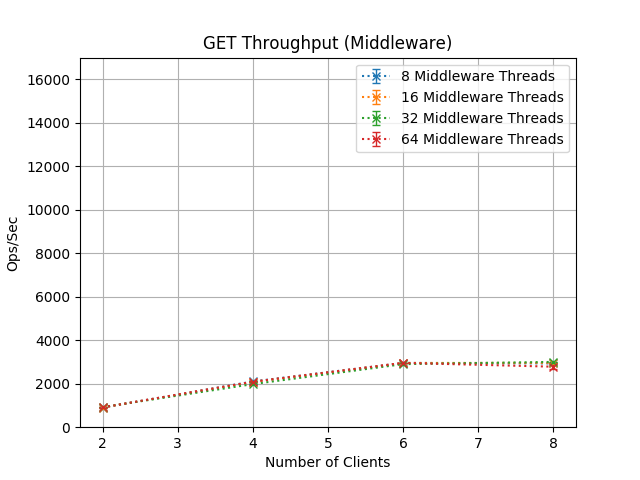
\includegraphics[width=\textwidth]{../illustrations/plots/2_2_1_two_middlewares_reduced/0-1/middleware_get_tp_s.png}
        \caption{\texttt{GET} Throughput}
        \label{fig:two_middlewares_reduced_get_tp_mw}
    \end{minipage}\hfill
    \begin{minipage}{0.5\textwidth}
        \centering
        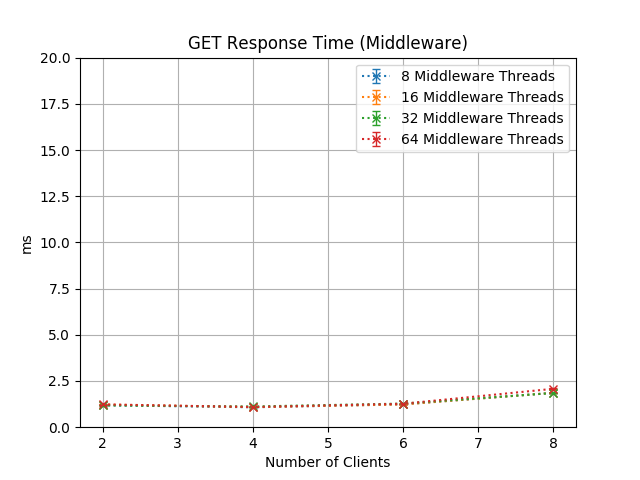
\includegraphics[width=\textwidth]{../illustrations/plots/2_2_1_two_middlewares_reduced/0-1/middleware_get_rt_ms.png}
        \caption{\texttt{GET} Response Time}
        \label{fig:two_middlewares_reduced_get_rt_mw}
    \end{minipage}
\end{figure}
%
As we can rather clearly see the system gets saturated after 6 total clients, supporting the conclusions above that the system is saturated during the whole experiment, since we start at 6 clients in total.
%
\subsection{Summary}
%
\begin{center}
	{Maximum throughput for one middleware.}
	\begin{tabular}{|l|p{2cm}|p{2cm}|p{2cm}|p{2cm}|}
		\hline                                & Throughput & Response time & Average time in queue & Miss rate \\ 
		\hline Reads: Measured on middleware  &   2621     &     1.27 ms   &         0.1 ms        &   1.3 \%  \\ 
		\hline Reads: Measured on clients     &   2606     &     2.31 ms   & n/a                   &   1.3 \%  \\ 
		\hline Writes: Measured on middleware &  13045     &     4.54 ms   &         1.07 ms       & n/a       \\ 
		\hline Writes: Measured on clients    &  12976     &     9.33 ms   & n/a                   & n/a       \\ 
		\hline 
	\end{tabular}
\end{center}
%
What is interesting in this table is that the response time measured on the client is significantly higher than the response time measured on the middleware.
%
On the middleware we measured the response time from the moment the socket was ready to be read from to the moment we finished processing the request, i.e. including the time the request needs to be written to the socket.
%
When checking the response time measured by memtier we can quickly see that there is an anomaly in the plot and the response time using 96 clients is an outlier.
%
The plot for this is included in the repository but omitted in the report.
%
\begin{center}
	{Maximum throughput for two middlewares.}
	\begin{tabular}{|l|p{2cm}|p{2cm}|p{2cm}|p{2cm}|}
		\hline                                & Throughput & Response time & Average time in queue & Miss rate \\ 
		\hline Reads: Measured on middleware  &   2686     &     1.20 ms   &          0.07 ms      & 0,9 \%    \\ 
		\hline Reads: Measured on clients     &   2673     &     2.25 ms   & n/a                   & 0,9 \%    \\ 
		\hline Writes: Measured on middleware &   17290    &     9.29 ms   &           2.45 ms     & n/a       \\ 
		\hline Writes: Measured on clients    &   17187    &     13.69 ms  & n/a                   & n/a       \\ 
		\hline 
	\end{tabular}
\end{center}
%
Again here we see an outlier in the measurements on the client, again the plot is included in the repository.
%
\par
%
In both tables the throughput measured by the client is slightly different than the one measured in the middleware, this is because we use histograms binned to one second to compute the average throughput.
%
Since we have a network between the client machines and the middlewares we do not expect to get the exact same bins.
%
\par
%
First we can see that the response time on the client is always larger than the response time measured on the middleware, this is a very simple sanity check on the data.
%
Further we can see that we cannot increase the throughput for \texttt{GET} requests when adding a second middleware, which confirms the conclusion made before that memcached is the bottleneck in this case.
%
The response time for \texttt{GET} requests also behaves similarly for both settings, which supports the fact that the response time is mainly due to memcached, which can also be seen by the negligible queue wait time.
%
\par
%
When we look at \texttt{SET} requests however the behaviour is very different.
%
First we can see that in fact we can saturate the memcached server, by comparing the throughput with the throughput table from the first experiment.
%
Second we can see that adding a second middleware increases the throughput significantly, which supports the above conclusion that in the first case the middleware is the bottleneck.
%
When comparing the response times we can see that adding a middleware increases the response times for writes significantly, this can be explained by the fact that memcached is handling a lot more requests.
%
As we have seen in previous experiments the service time of memcached increases even in an undersaturated setting, but certainly so when saturated.
%
\par
%
In general we can say that there were no real surprises, the behaviour of the system is consistent with what we have seen up to now.
%
\section{Throughput for Writes (90 pts)}\label{sec:tp_write}
%
\subsection{Full System}
%
\subsubsection{System Setup}
%
For this experiment we will use the following system setup:
%
\begin{itemize}
	\item 3 client machines with 2 memtier instances per machine. Each instance of memtier runs with 1 threads.
	\item 2 middlewares
	\item 3 memcached servers
\end{itemize}
%
We vary the number of virtual clients per thread from 1 to 48.
%
\subsubsection{Hypothesis}
%
This is the first experiment where the middleware has to coordinate across multiple servers.
%
We therefore expect a smaller throughput for \texttt{SET} requests for the full system than the configuration in the previous experiment.
%
The reason is that inside the middleware, when handling \texttt{SET} requests the request is first sent to all three servers and then waited for.
%
That means we generate a small overhead by having three send and read operations, this overhead should make itself visible in the throughput of the system.
%
\subsubsection{Explanation}
%
\begin{figure}[H]
	\centering
	\captionsetup{width=0.4\textwidth}
    \begin{minipage}{0.5\textwidth}
        \centering
        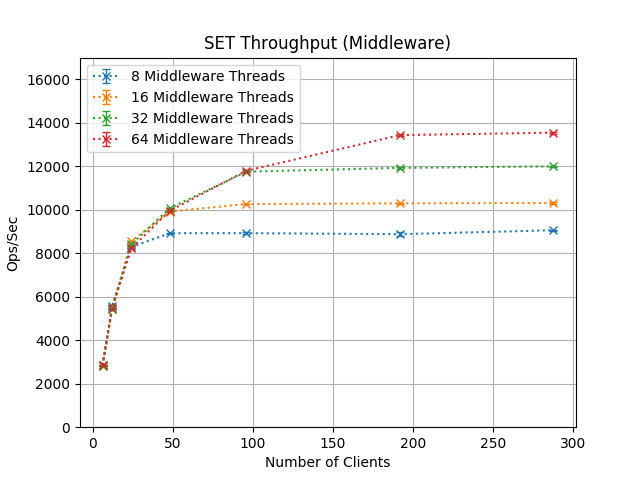
\includegraphics[width=\textwidth]{../illustrations/plots/3_1_full_system_write/1-0/middleware_set_tp_s.png}
        \caption{\texttt{SET} Throughput}
        \label{fig:full_system_write_set_tp_mw}
    \end{minipage}\hfill
    \begin{minipage}{0.5\textwidth}
        \centering
        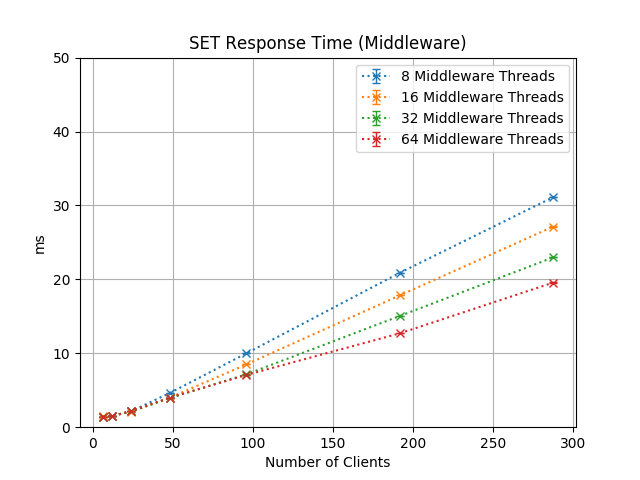
\includegraphics[width=\textwidth]{../illustrations/plots/3_1_full_system_write/1-0/middleware_set_rt_ms.png}
        \caption{\texttt{SET} Response Time}
        \label{fig:full_system_write_set_rt_mw}
    \end{minipage}
\end{figure}
%
\begin{figure}[H]
	\centering
	\captionsetup{width=0.4\textwidth}
    \begin{minipage}{0.5\textwidth}
        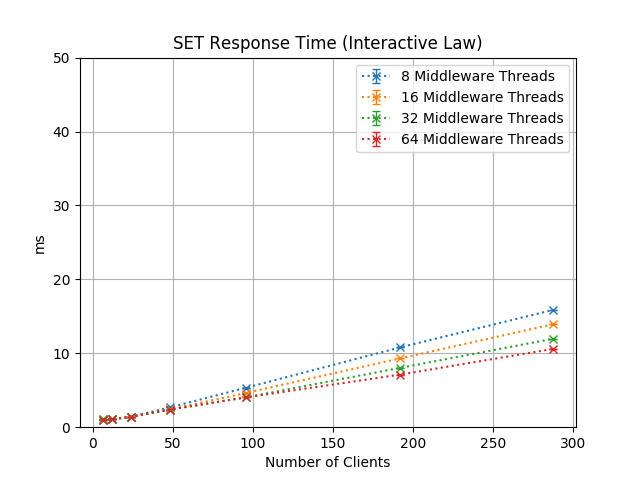
\includegraphics[width=\textwidth]{../illustrations/plots/3_1_full_system_write/1-0/middleware_interactive_set_rt_ms.png}
        \caption{\texttt{SET} Response time IRTL}
        \label{fig:full_system_write_set_rt_it}
    \end{minipage}\hfill
\end{figure}
%
\begin{figure}[H]
	\centering
	\captionsetup{width=0.4\textwidth}
    \begin{minipage}{0.5\textwidth}
        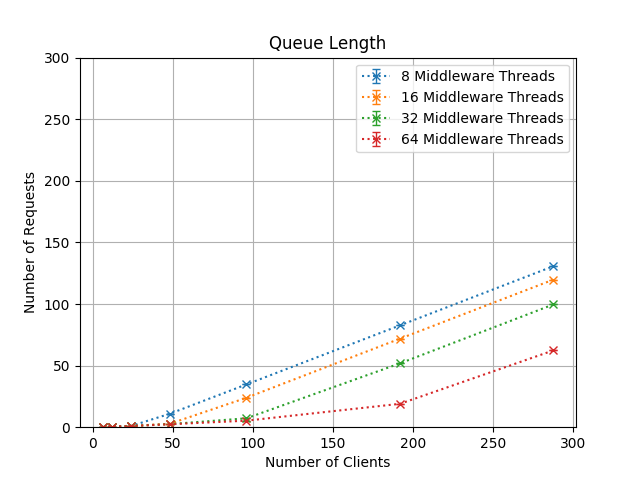
\includegraphics[width=\textwidth]{../illustrations/plots/3_1_full_system_write/1-0/middleware_queue_length.png}
        \caption{\texttt{SET} Queue Length}
        \label{fig:full_system_write_set_ql}
    \end{minipage}\hfill
    \begin{minipage}{0.5\textwidth}
        \centering
        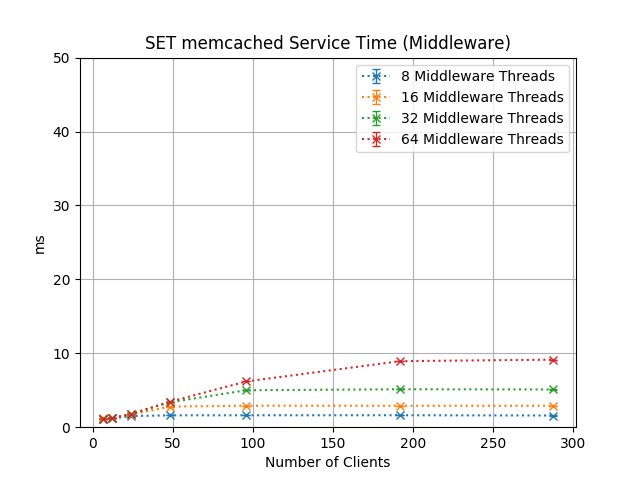
\includegraphics[width=\textwidth]{../illustrations/plots/3_1_full_system_write/1-0/middleware_set_service_time_ms.png}
        \caption{\texttt{SET} Service Time of memcached}
        \label{fig:full_system_write_set_st_mw}
    \end{minipage}
\end{figure}
%
As we can see very nicely in Figure~\ref{fig:full_system_write_set_tp_mw} we can saturate the system for each configuration of worker threads.
%
Specifically it needs 24 clients for 8 threads, 48 clients for 16 threads, 96 clients for 32 threads and finally 192 clients for 64 threads.
%
The same thing can be seen in Figure~\ref{fig:full_system_write_set_rt_mw} showing that the slope of the response time increases for each worker thread configuration at the same thresholds as mentioned before.
%
Also we know from previous experiments a memcached server can handle up to approximately 17000 ops/sec.
%
In this case we reach a maximum of nearly 14000 ops/sec using 64 threads.
%
This is a first indication that the middlewares are the bottleneck of the system.
%
However Figure~\ref{fig:full_system_write_set_st_mw} shows similar behaviour of the memcached server as in the previous experiment when the server became the bottleneck which can be seen in Figure~\ref{fig:one_middleware_get_st_mw}
%
But we need to be careful here, since in Figure~\ref{fig:one_middleware_get_st_mw} we measure response times that are a lot higher than in this case.
%
That supports the suspicion that the middleware is the bottleneck of the system.
%
As a last confirmation we can again look at the queue length in Figure~\ref{fig:full_system_write_set_ql} where we can see that the requests begin to wait in the queue when the middlewares are saturated.
%
This supports the hypothesis made that the middleware has an overhead for coordinating \texttt{SET} requests across multiple servers.
%
We can further see that the more clients and less threads we use, the queue gets longer and longer, which explains the increase in response time, even if the server is not saturated.
%
Oversaturation does not occur in this experiment.
%
\subsection{Summary}
%
\begin{center}
	{Maximum throughput for the full system}
	\begin{tabular}{|l|p{1.5cm}|p{1.5cm}|p{1.5cm}|p{1.5cm}|}
		\hline                                            & WT=8 & WT=16 & WT=32 & WT=64 \\ 
		\hline Throughput (Middleware)                    &  8290    &  9920    &   11753   &   13435   \\ 
		\hline Throughput (Derived from MW response time) &  11046   &  12031   &   13412   &   15117   \\ 
		\hline Throughput (Client)                        &  8254    &  9865    &   11693   &   13365   \\ 
		\hline Average time in queue                      &  0.45 ms &  0.96 ms &   1.89 ms &   3.44 ms \\ 
		\hline Average length of queue                    &  1.04    &  2.78    &   7.23    &   18.99   \\ 
		\hline Average time waiting for memcached         &  1.51 ms &  2.79 ms &   5.00 ms &   8.93 ms \\ 
		\hline 
	\end{tabular}
	\label{max_tp_table}
\end{center}
%
Same as before the values in the table do not completely reflect the absolute maximum throughput recorded.
%
The numbers are the throughput recorded when the system goes into the saturation phase.
%
The absolute maximum throughput is not an accurate representation of the performance of the system.
%
\par
%
The derived throughput is calculated as $X = N / R$, where $X$ is the derived throughput, $N$ the number of clients, and $R$ the response time.
%
\par
%
Overall we can say the system behaves as expected.
%
As we have seen before two middlewares can handle up to 192 clients before being saturated with \texttt{SET} requests, here we see the same thing, however now the workers have a slight overhead, so the throughput that they produce is lower.
%
Increasing the worker threads also increases the throughput.
%
However when doubling the worker threads the throughput does not double as well.
%
This is due to the fact the the middleware is not completely parallelized, therefore we have diminishing returns in terms of throughput and adding more worker threads.
%
\par
%
Looking at the derived throughput we can quickly see that the this estimation is higher than the actual measured throughput.
%
This has to do with the fact that we derive this throughput based on the response time we measure on the middleware, this does not take into account the latency of the requests between the client machines and the middlewares.
%
Other than that also here we can see that the throughput increases with the number of worker threads.
%
\par
%
The throughput measured on the clients is also slightly different from the throughput we measured on the middleware. 
%
This is due to the fact that the binning for the throughput histograms per second is done based on two different measurements.
%
However this is to be expected and as long as the difference is insignificant as it is there is no problem with that.
%
\par
%
Further we can see that when we increase the number of worker threads the waiting time for memcached increases as well.
%
This is explained by the fact that the more threads are running in the middlewares, the more requests are concurrently sent to memcached.
%
\par
%
This fact directly influences the time in queue as well as the queue length.
%
The longer requests are being processed by memcached, the longer the worker threads need to wait for a response.
%
That means that the requests need to wait longer in the queue before being dequeued by a worker, which in turn explains the increase in queue size.
%
All in all there are no real surprises, the system behaves as we would it expect to behave.

\section{Gets and Multi-gets (90 pts)}
%
\subsection{Sharded Case}
%
\subsubsection{System Setup}
%
For this experiment we will use the following system setup:
%
\begin{itemize}
	\item 3 client machines with 2 memtier instances per machine. Each instance of memtier runs with 1 threads.
	\item 2 middlewares
	\item 3 memcached servers
\end{itemize}
%
We will use 2 virtual clients per thread in all the configurations.
%
We will vary the multi-get size in the workload from 1 to 12.
%
\subsubsection{Hypothesis}
%
In this scenario we will be splitting the keys if we encounter more than one key in a \texttt{GET} requests.
%
Therefore we expect the response time to be almost constant, as long as the key size is smaller or equal to the number of servers.
%
Other than that the system should behave similarly to a normal \texttt{GET} workload, since at some point we should saturate the servers and then the response time should increase linearly again.
%
\subsubsection{Explanation}
%
\begin{figure}[H]
	\centering
	\captionsetup{width=0.4\textwidth}
    \begin{minipage}{0.5\textwidth}
        \centering
        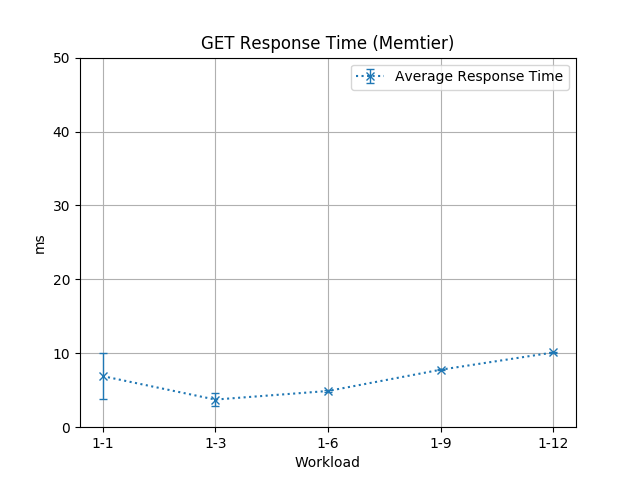
\includegraphics[width=\textwidth]{../illustrations/plots/4_1_full_system_read_sharded/64/memtier_get_rt_ms.png}
        \caption{\texttt{GET} Response Time sharded (MT)}
        \label{fig:full_system_read_sharded_mt_rt}
    \end{minipage}\hfill
    \begin{minipage}{0.5\textwidth}
        \centering
        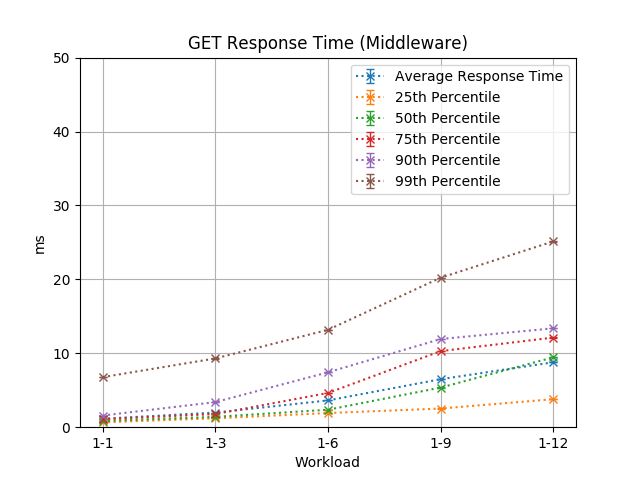
\includegraphics[width=\textwidth]{../illustrations/plots/4_1_full_system_read_sharded/64/middleware_get_rt_ms.png}
        \caption{\texttt{GET} Response Time sharded (MW)}
        \label{fig:full_system_read_sharded_mw_rt}
    \end{minipage}
\end{figure}
%
\begin{figure}[H]
	\centering
	\captionsetup{width=0.4\textwidth}
    \begin{minipage}{0.5\textwidth}
        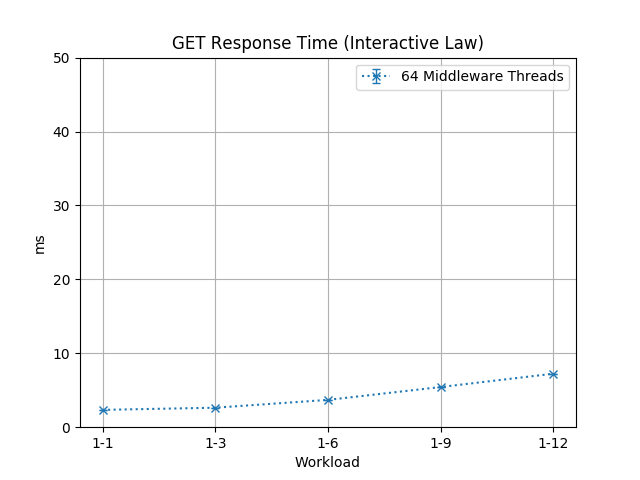
\includegraphics[width=\textwidth]{../illustrations/plots/4_1_full_system_read_sharded/64/middleware_interactive_get_rt_ms.png}
        \caption{\texttt{GET} Response time IRTL}
        \label{fig:full_system_read_sharded_mw_rt_it}
    \end{minipage}\hfill
    \begin{minipage}{0.5\textwidth}
        \centering
        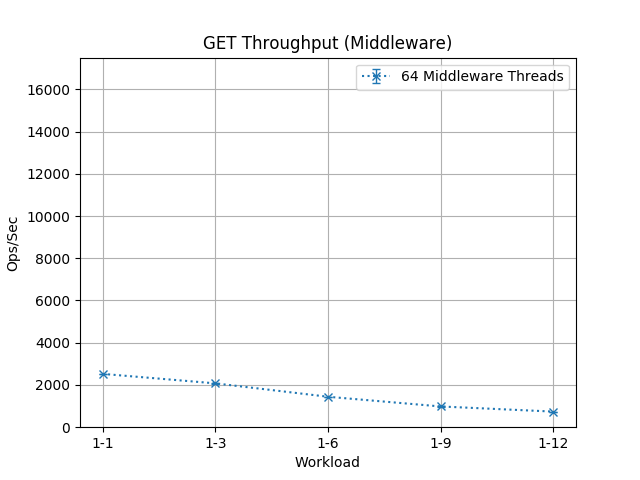
\includegraphics[width=\textwidth]{../illustrations/plots/4_1_full_system_read_sharded/64/middleware_get_tp_s.png}
        \caption{\texttt{GET} Throughput sharded}
        \label{fig:full_system_read_sharded_mw_tp}
    \end{minipage}
\end{figure}
%
\begin{figure}[H]
	\centering
	\captionsetup{width=0.4\textwidth}
    \begin{minipage}{0.5\textwidth}
        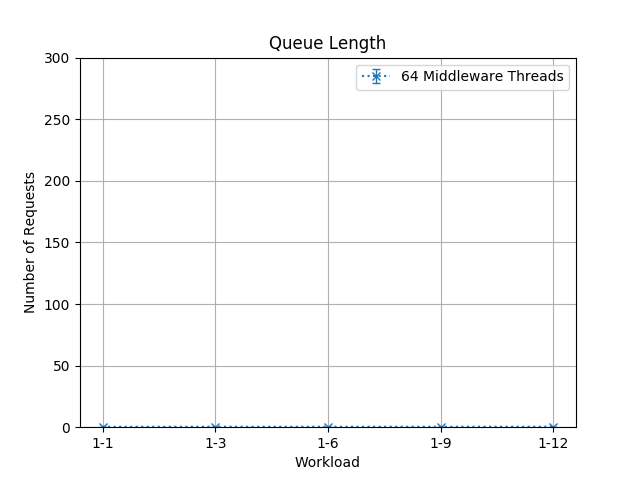
\includegraphics[width=\textwidth]{../illustrations/plots/4_1_full_system_read_sharded/64/middleware_queue_length.png}
        \caption{\texttt{GET} Queue Length}
        \label{fig:full_system_read_sharded_mw_ql}
    \end{minipage}\hfill
    \begin{minipage}{0.5\textwidth}
        \centering
        \includegraphics[width=\textwidth]{../illustrations/plots/4_1_full_system_read_sharded/64/middleware_get_service_time_ms.png}
        \caption{\texttt{GET} Service Time of memcached}
        \label{fig:full_system_read_sharded_mw_st}
    \end{minipage}
\end{figure}
%
In Figure~\ref{fig:full_system_read_sharded_mt_rt} we can see that the first two datapoints have rather large errors.
%
Since the response time in the middleware is rather stable, and the measurement for the response time in the middleware is end to and we can attribute these errors to inconsistencies in the network connecting the client machines and middlewares.
%
These outliers do not really affect the argumentation below, but I wanted to mention this fact anyways.
%
\par
%
First let us look at the throughput in Figure~\ref{fig:full_system_read_sharded_mw_tp}.
%
We can see that when increasing the multi-get key size the throughput decreases, which is rather straight forward, since we are requesting more keys per request, even if sharding is enabled.
%
In the middleware we try to distribute a \texttt{MULTI-GET} request as equally as possible to the servers.
%
\par
%
When looking at Figure~\ref{fig:full_system_read_sharded_mw_ql} we can see that for all key sizes, the queue stays empty, therefore we can conclude that we do not saturate the middlewares using these configurations.
%
Usually this means that the server is the bottleneck, since 12 total clients in this case on 3 client machines can easily generate enough requests to saturate the servers, as we have seen numerous times in previous experiments.
%
We can confirm this suspicion when looking at the service time of the memcached servers in Figure~\ref{fig:full_system_read_sharded_mw_st}.
%
\par
%
Until we have 3 keys per request the service time is stable, which is to be expected, since we can distribute the requests across mutliple servers, meaning 3 keys should have the same response time as 1 key, with a small overhead for the coordination across the servers, parsing and splitting the command.
%
After this point the service time starts to increase linearly, which indicates that the servers are getting saturated.
%
From previous experiments we know that we can support approximately 3000 read ops/sec on one server, when retrieving one key.
%
In section~\ref{subsec:two_middlewares_explanation} we learned that 2 servers can handle up to approximately 6000 single key \texttt{GET} requests per second. 
%
Therefore it is resonable to assume that three servers should be able to handle up to 9000 ops/sec.
%
This can be confirmed by again looking at the throughput plot.
%
After 6 keys per request multiplying the multi-get key size with the number of requests processed per second matches the maximum of approximately 9000 ops/sec.
%
Which again supports the conclusion that the memcached servers are saturated.
%
\par
%
In Figure~\ref{fig:full_system_read_sharded_mw_rt} and Figure~\ref{fig:full_system_read_sharded_mw_st} see that the increase in response time is mainly due to the increase in service time, therefore we can assume that sharding the command does a small but constant overhead to the processing of the request.
%
Further we can compare Figure~\ref{fig:full_system_read_sharded_mw_rt} with Figure~\ref{fig:full_system_read_sharded_mt_rt} and see that the network does also not contribute a significant increase in response time, since the difference between the measured response time in the middleware and memtier is more or less constant.
%
\subsection{Non-sharded Case}
%
\subsubsection{System Setup}
%
For this experiment we will use the following system setup:
%
\begin{itemize}
	\item 3 client machines with 2 memtier instances per machine. Each instance of memtier runs with 1 threads.
	\item 2 middlewares
	\item 3 memcached servers
\end{itemize}
%
We will use 2 virtual clients per thread in all the configurations.
%
We will vary the multi-get size in the workload from 1 to 12.
%
\subsubsection{Hypothesis}
%
In this case we do not shard commands, therefore the system should behave a little differently.
%
Since we do not process the requests and treat them the same way as \texttt{GET} requests, i.e. send them only to one server, we expect to see lower response times than in the sharded mode with small request sizes
%
However with larger requests we expect again the servers to be the main reason for the increase in response time, as we have seen above.
%
\subsubsection{Explanation}
%
\begin{figure}[H]
	\centering
	\captionsetup{width=0.4\textwidth}
    \begin{minipage}{0.5\textwidth}
        \centering
        \includegraphics[width=\textwidth]{../illustrations/plots/4_2_full_system_read/64/memtier_get_rt_ms.png}
        \caption{\texttt{GET} Response Time non-sharded (MT)}
        \label{fig:full_system_read_mt_rt}
    \end{minipage}\hfill
    \begin{minipage}{0.5\textwidth}
        \centering
        \includegraphics[width=\textwidth]{../illustrations/plots/4_2_full_system_read/64/middleware_get_rt_ms.png}
        \caption{\texttt{GET} Response Time non-sharded (MW)}
        \label{fig:full_system_read_mw_rt}
    \end{minipage}
\end{figure}
%
\begin{figure}[H]
	\centering
	\captionsetup{width=0.4\textwidth}
    \begin{minipage}{0.5\textwidth}
        \includegraphics[width=\textwidth]{../illustrations/plots/4_2_full_system_read/64/middleware_interactive_get_rt_ms.png}
        \caption{\texttt{GET} Response time IRTL}
        \label{fig:full_system_read_mw_rt_it}
    \end{minipage}\hfill
    \begin{minipage}{0.5\textwidth}
        \centering
        \includegraphics[width=\textwidth]{../illustrations/plots/4_2_full_system_read/64/middleware_get_tp_s.png}
        \caption{\texttt{GET} Throughput non-sharded}
        \label{fig:full_system_read_mw_tp}
    \end{minipage}
\end{figure}
%
\begin{figure}[H]
	\centering
	\captionsetup{width=0.4\textwidth}
    \begin{minipage}{0.5\textwidth}
        \includegraphics[width=\textwidth]{../illustrations/plots/4_2_full_system_read/64/middleware_queue_length.png}
        \caption{\texttt{GET} Queue Length}
        \label{fig:full_system_read_mw_ql}
    \end{minipage}\hfill
    \begin{minipage}{0.5\textwidth}
        \centering
        \includegraphics[width=\textwidth]{../illustrations/plots/4_2_full_system_read/64/middleware_get_service_time_ms.png}
        \caption{\texttt{GET} Service Time of memcached}
        \label{fig:full_system_read_mw_st}
    \end{minipage}
\end{figure}
%
As we can quickly see when looking at Figure~\ref{fig:full_system_read_mw_ql} also in this case the middleware does not get saturated, the argumentation for this is the same as before.
%
Thus we again expect the servers to be the bottleneck of the system, for this we look at the service time in Figure~\ref{fig:full_system_read_mw_st}.
%
There we can see that after a workload of 3 keys per request the service time starts to increase linearly.
%
This is one indication that the server is the bottleneck sometime after 3 keys per request. 
%
Further in Figure~\ref{fig:full_system_read_mw_tp} we can see that with a workload of of 6 keys per request the throughout is approximately 9000 ops/sec, which corresponds with what we learned in previous experiments, that with 3 servers we can handle approximately 9000 single key requests per second.
%
This means that at 6 keys per request the servers are saturated, which supports the above conclusion.
%
Again we can see that the service time accounts for most of the increase in the response time, which in this case is to be expected since the middleware just relays messages between the clients and the servers.
%
Also again we can confirm that the network is not adding significantly to the response time for larger resquests, as we have seen in the sharded case.
%
\subsection{Histogram}
%
In Figures~\ref{fig:full_system_sharded_read_mt_hist}-\ref{fig:full_system_read_mw_hist} we can see the histograms of response times for a workload of 6 keys per request.
%
\par
%
In the case of the middleware the construction is rather simple, we just record the response time for all requests and then plot a histogram of those.
%
\par
%
In the case of memtier it is a bit more difficult since the output of memtier does not give us the same data as the middleware.
%
At the end of each run of memtier we receive a cumulative distribution of the response times, meaning each line tells us how many percent of requests have a response time smaller than the mentioned response time on the respective line.
%
Using this distribution we can calculate how many percent of requests fall between two specific values of response time.
%
We aggregate this data over all clients and runs, using this we can plot a histogram.
%
\par
%
Since the two systems do not provide us with the same type of data (number of requests vs. percentage) we can plot the histograms on a normalized y-axis, since normalization does not change the shape of histograms.
%
Further we capped the response time at 20 msec, since the outliers would make the histograms unreadable.
%
For all histograms we use 40 bins, therefore making one bin 0.5 msec wide.
%
\begin{figure}[H]
	\centering
	\captionsetup{width=0.4\textwidth}
    \begin{minipage}{0.5\textwidth}
        \centering
        \includegraphics[width=\textwidth]{../illustrations/plots/4_1_full_system_read_sharded/64/memtier_get_hist.png}
        \caption{\texttt{GET} Histogram sharded mode (MT)}
        \label{fig:full_system_sharded_read_mt_hist}
    \end{minipage}\hfill
    \begin{minipage}{0.5\textwidth}
        \centering
        \includegraphics[width=\textwidth]{../illustrations/plots/4_1_full_system_read_sharded/64/middleware_get_hist.png}
        \caption{\texttt{GET} Histogram sharded mode (MW)}
        \label{fig:full_system_sharded_read_mw_hist}
    \end{minipage}
\end{figure}
%
\begin{figure}[H]
	\centering
	\captionsetup{width=0.4\textwidth}
    \begin{minipage}{0.5\textwidth}
        \centering
        \includegraphics[width=\textwidth]{../illustrations/plots/4_2_full_system_read/64/memtier_get_hist.png}
        \caption{\texttt{GET} Histogram non-sharded mode (MT)}
        \label{fig:full_system_read_mt_hist}
    \end{minipage}\hfill
    \begin{minipage}{0.5\textwidth}
        \centering
        \includegraphics[width=\textwidth]{../illustrations/plots/4_2_full_system_read/64/middleware_get_hist.png}
        \caption{\texttt{GET} Histogram non-sharded mode (MW)}
        \label{fig:full_system_read_mw_hist}
    \end{minipage}
\end{figure}
%
\subsection{Summary}
%
Let us start by comparing the histograms above, the allow us to draw a direct comparison between running the middleware in sharded and non-sharded mode.
%
First we can see that the response times measured in the middleware are smaller than the ones measured in memtier, this is of course to be expected, since the middleware does not include the network latency between the VMs.
%
By comparing Figure~\ref{fig:full_system_sharded_read_mw_hist} with Figure~\ref{fig:full_system_read_mw_hist} we can determine that sharding does not seem to help with processing of the request. 
%
We can see that with sharding enabled the amount of requests that have a higher than average response time increases.
%
This can be confirmed by looking at Figure~\ref{fig:full_system_read_mw_rt} and comparing it with Figure~\ref{fig:full_system_read_sharded_mw_rt}.
%
\par
%
In the former the 50th percentile is significantly lower than the average response time, whereas with sharding enabled we see that the median is even larger than the average response time in the latter.
%
Further we can see that the average response time in the sharded case is even higher than in the non-sharded case, which further shows that sharding does not really make sense in this setting.
%
This indicates that sharding the command sending it to different servers and then reassembling it in the middleware adds an overhead that is not compensated by distributing the load across multiple servers.
%
In principle this tells us that the implementation of memcached is rather resilient to retrieving multiple keys, at least for the tested range.
%
\par
%
In principle it might be a bit counterintuitive that sharded and non sharded mode are behaving so similarly and are saturated at the same points.
%
However when we interpret the throughput differently, namely as how many keys per second does the server need to retrieve the values for both modes are approximately the same.
%
The difference is just that in the sharded mode the server retrieves multiple smaller requests and in non-sharded larger ones, but the number of keys stays approximately the same.
%
\section{2K Analysis (90 pts)}
%
\subsection{System Setup}
%
For this experiment we will use the following system setup:
%
\begin{itemize}
	\item 3 client machines with 2/1 memtier instances per machine. Each instance of memtier runs with 1/2 threads.
	\item 2/1 middlewares
	\item 3/1 memcached servers
\end{itemize}
%
We will run each combination of the mentioned configurations.
%
Further we will use 8 and 32 threads in the middleware for each configuration.
%
We will use 32 virtual clients per thread in all configurations.
%
Also we will run a read-only and a write-only workload.
%
\subsection{Parameter Definitions}
%
We mentioned in the previous subsection which parameters we are going to test.
%
In the following table we can see a summary of that:
%
\begin{table}[H]
\centering
\begin{tabular}{|c|c|c|c|}
\hline Factor & Shortname & -1 & +1\\
\hline
\hline Worker Threads & WT & 8 & 32\\
\hline Memcached Servers & MC & 1 & 3 \\
\hline Middlewares & MW & 1 & 2\\
\hline
\end{tabular}
\caption{Parameter Definitions}
\end{table}
%
We will refer to the parameters in the following tables only by their shortnames.
%
Further combinations of parameters will be combined using a *, for example combining the effects of the worker threads and the memcached server will be referred as WT*MC.
%
Using these parameters we will assume an additive model of different effects.
%
This leads to the following equation we would like to solve for each experiment:
\[
a + b \cdot MC + c \cdot MW + d \cdot WT + e \cdot MC \cdot MW + f \cdot MC \cdot WT + g \cdot MW \cdot WT + h \cdot MC \cdot MW \cdot WT = Y
\]
%
Where $Y$ corresponds to either throughput or response time.
%
For each experiment we will setup a table and then compute the effects using the sign table method.
%
We can use these effects to compute the part of the variation that is explained by each of the variables, and then based on these numbers make conclusions on what has the most influence on our throughput respectively our response time.
%
For each experiment we will setup the sign tables for throughput and response time, fill in the results from the experiments and compute the effects.
%
Using the effects we can calculate the allocation of variation directly.
%
\subsection{Write-only workload}
%
\begin{table}[H]
\centering
\scriptsize{
\begin{tabular}{|c|c|c|c|c|}
\hline MW & MC & WT & Avg. TP (ops/sec) & Avg. RT (ms)\\
\hline
-1 & -1 & -1 & 5616.83 & 33.12\\
\hline
-1 & -1 & 1 & 9514.23 & 17.71\\
\hline
1 & -1 & -1 & 7264.69 & 21.00\\
\hline
1 & -1 & 1 & 11776.94 & 14.62\\
\hline
-1 & 1 & -1 & 4035.64 & 38.35\\
\hline
-1 & 1 & 1 & 7010.56 & 24.48\\
\hline
1 & 1 & -1 & 5993.84 & 29.86\\
\hline
1 & 1 & 1 & 9174.76 & 18.41\\
\hline
\end{tabular}
}
\caption{Write-Only Workload}
\end{table}
%
\begin{table}[H]
\centering
\scriptsize{
\begin{tabular}{|c|ccccccc|c|}
\hline I & MW & MC & WT & MW*MC & MW*WT & MC*WT & MW*MC*WT & Avg. TP (ops/sec)\\
\hline
1 & -1 & -1 & -1 & 1 & 1 & 1 & -1 & 5616.83\\
1 & -1 & -1 & 1 & 1 & -1 & -1 & 1 & 9514.23\\
1 & 1 & -1 & -1 & -1 & -1 & 1 & 1 & 7264.69\\
1 & 1 & -1 & 1 & -1 & 1 & -1 & -1 & 11776.94\\
1 & -1 & 1 & -1 & -1 & 1 & -1 & 1 & 4035.64\\
1 & -1 & 1 & 1 & -1 & -1 & 1 & -1 & 7010.56\\
1 & 1 & 1 & -1 & 1 & -1 & -1 & -1 & 5993.84\\
1 & 1 & 1 & 1 & 1 & 1 & 1 & 1 & 9174.76\\
\hline
60387.49 & 8032.97 & -7957.88 & 14565.49 & 211.83 & 820.86 & -2253.80 & -408.86 & Total\\
7548.44 & 1004.12 & -994.74 & 1820.69 & 26.48 & 102.61 & -281.72 & -51.11 & Total/8\\
100.0\% & 18.65\% & 18.3\% & 61.32\% & 0.01\% & 0.19\% & 1.47\% & 0.05\% & Variation\\
\hline
\end{tabular}
}
\caption{Write-Only Workload Sign Table Avg. TP (ops/sec)}
\label{2k_set_tp}
\end{table}
%
\begin{table}[H]
\centering
\scriptsize{
\begin{tabular}{|c|ccccccc|c|}
\hline I & MW & MC & WT & MW*MC & MW*WT & MC*WT & MW*MC*WT & Avg. RT (ms)\\
\hline
1 & -1 & -1 & -1 & 1 & 1 & 1 & -1 & 33.12\\
1 & -1 & -1 & 1 & 1 & -1 & -1 & 1 & 17.71\\
1 & 1 & -1 & -1 & -1 & -1 & 1 & 1 & 21.00\\
1 & 1 & -1 & 1 & -1 & 1 & -1 & -1 & 14.62\\
1 & -1 & 1 & -1 & -1 & 1 & -1 & 1 & 38.35\\
1 & -1 & 1 & 1 & -1 & -1 & 1 & -1 & 24.48\\
1 & 1 & 1 & -1 & 1 & -1 & -1 & -1 & 29.86\\
1 & 1 & 1 & 1 & 1 & 1 & 1 & 1 & 18.41\\
\hline
197.55 & -29.77 & 24.66 & -47.11 & 0.67 & 11.45 & -3.54 & -6.61 & Total\\
24.69 & -3.72 & 3.08 & -5.89 & 0.08 & 1.43 & -0.44 & -0.83 & Total/8\\
100.0\% & 22.72\% & 15.58\% & 56.89\% & 0.01\% & 3.36\% & 0.32\% & 1.12\% & Variation\\
\hline
\end{tabular}
}
\caption{Write-Only Workload Sign Table Avg. RT (ms)}
\label{2k_set_rt}
\end{table}
%
First we will look at the throughput when using a write-only workload.
%
The corresponding computations are shown in Table~\ref{2k_set_tp}
%
As we can quickly see the largest portion of the variation happens when we increase the number of worker threads.
%
Also when doubling the number of middlewares we can increase the throughput.
%
We can explain the fact that increasing the number of workers claims so much of the variation by the fact that we quadruple the number of worker threads, but only double the number of workers when using 2 middlewares.
%
\par
%
As we can determine by the table adding a memcached server impacts the write throughput rather negatively.
%
This is pretty straight forward, since we know that the middleware must coordinate \texttt{SET} requests across multiple servers.
%
\par
%
Looking at Table~\ref{2k_set_rt} where we can see the variation attribution of the response time we can see similar effects.
%
Adding more workers and middlewares decreases the response time, again quadrupling the number of worker threads has much more impact than using two middlewares.
%
However when we add a second server the response time increases, which again can be explained by the overhead of replicating \texttt{SET} requests.
%
\par
%
Interesting to see is that the combined effects of the factors have almost no influence, on the response time or the throughput.
%
In the case of MW*MC it seems that using two middlewares directly cancels the overhead of replicating the requests to multiple servers.
%
We can also see that by increasing the middlewares and the worker threads we can gain a little more throughput than by using only one of the two.
%
The fact that the performance increase is so small is explained by the fact that in this case the single memcached server is saturated by the many worker threads.
%
This in turn explains the increase in response time, since saturating the server will increase the service time of the server, which directly impacts the response time of the system.
%
\par
%
In general the findings above correspond to what we have seen in the previous experiments.
%
We saw in section~\ref{subsec:two_middlewares_explanation} that we can saturate the servers using two middlewares and in section~\ref{subsec:one_middleware_explanation} that one middleware is not enough.
%
That is why we can gain so much performance by adding a middleware or more worker threads.
%
\subsection{Read-only workload}
%
\begin{table}[H]
\centering
\scriptsize{
\begin{tabular}{|c|c|c|c|c|}
\hline MW & MC & WT & Avg. TP (ops/sec) & Avg. RT (ms)\\
\hline
-1 & -1 & -1 & 2987.82 & 63.30\\
\hline
-1 & -1 & 1 & 2939.13 & 64.02\\
\hline
1 & -1 & -1 & 3005.22 & 62.47\\
\hline
1 & -1 & 1 & 3007.24 & 61.73\\
\hline
-1 & 1 & -1 & 8568.48 & 21.17\\
\hline
-1 & 1 & 1 & 9071.78 & 19.84\\
\hline
1 & 1 & -1 & 8967.35 & 19.64\\
\hline
1 & 1 & 1 & 9009.09 & 19.66\\
\hline
\end{tabular}
}
\caption{Read-Only Workload}
\end{table}
%
\begin{table}[H]
\centering
\scriptsize{
\begin{tabular}{|c|ccccccc|c|}
\hline I & MW & MC & WT & MW*MC & MW*WT & MC*WT & MW*MC*WT & Avg. TP (ops/sec)\\
\hline
1 & -1 & -1 & -1 & 1 & 1 & 1 & -1 & 2987.82\\
1 & -1 & -1 & 1 & 1 & -1 & -1 & 1 & 2939.13\\
1 & 1 & -1 & -1 & -1 & -1 & 1 & 1 & 3005.22\\
1 & 1 & -1 & 1 & -1 & 1 & -1 & -1 & 3007.24\\
1 & -1 & 1 & -1 & -1 & 1 & -1 & 1 & 8568.48\\
1 & -1 & 1 & 1 & -1 & -1 & 1 & -1 & 9071.78\\
1 & 1 & 1 & -1 & 1 & -1 & -1 & -1 & 8967.35\\
1 & 1 & 1 & 1 & 1 & 1 & 1 & 1 & 9009.09\\
\hline
47556.11 & 421.69 & 23677.31 & 498.38 & 250.67 & -410.85 & 591.70 & -512.28 & Total\\
5944.51 & 52.71 & 2959.66 & 62.30 & 31.33 & -51.36 & 73.96 & -64.04 & Total/8\\
100.0\% & 0.03\% & 99.77\% & 0.04\% & 0.01\% & 0.03\% & 0.06\% & 0.05\% & Variation\\
\hline
\end{tabular}
}
\caption{Read-Only Workload Sign Table Avg. TP (ops/sec)}
\label{2k_get_tp}
\end{table}
%
\begin{table}[H]
\centering
\scriptsize{
\begin{tabular}{|c|ccccccc|c|}
\hline I & MW & MC & WT & MW*MC & MW*WT & MC*WT & MW*MC*WT & Avg. RT (ms)\\
\hline
1 & -1 & -1 & -1 & 1 & 1 & 1 & -1 & 63.30\\
1 & -1 & -1 & 1 & 1 & -1 & -1 & 1 & 64.02\\
1 & 1 & -1 & -1 & -1 & -1 & 1 & 1 & 62.47\\
1 & 1 & -1 & 1 & -1 & 1 & -1 & -1 & 61.73\\
1 & -1 & 1 & -1 & -1 & 1 & -1 & 1 & 21.17\\
1 & -1 & 1 & 1 & -1 & -1 & 1 & -1 & 19.84\\
1 & 1 & 1 & -1 & 1 & -1 & -1 & -1 & 19.64\\
1 & 1 & 1 & 1 & 1 & 1 & 1 & 1 & 19.66\\
\hline
331.82 & -4.84 & -171.21 & -1.33 & 1.42 & -0.11 & -1.28 & 2.80 & Total\\
41.48 & -0.61 & -21.40 & -0.17 & 0.18 & -0.01 & -0.16 & 0.35 & Total/8\\
100.0\% & 0.08\% & 99.87\% & 0.01\% & 0.01\% & 0.0\% & 0.01\% & 0.03\% & Variation\\
\hline
\end{tabular}
}
\caption{Read-Only Workload Sign Table Avg. RT (ms)}
\label{2k_get_rt}
\end{table}
%
In this case, when using a read-only workload, the system behaves a lot differently.
%
All the factors have negligible impact on the performance of the system except increasing the number of servers.
%
As we have seen in the previous experiments, specifcally section~\ref{subsec:one_middleware_explanation} and~\ref{subsec:two_middlewares_explanation} one memcached server is saturated rather quickly when issuing \texttt{GET} requests.
%
Therefore it makes sense that as long as we do not widen this bottleneck the system cannot start performing better.
%
But as soon as we do exactly that the performance spikes.
%
\par
%
The same can be seen in Table~\ref{2k_get_rt} with the response time, where increasing the number of memcached servers drastically reduces the response time.
%
This is due to the fact that the middleware can load balance read requests across multiple memcached servers.
%
In this case adding a server does not add more work for the middleware, but we can saturate up to 3 memcached servers.
%
This again can be seen by looking at the throughput, using 3 servers we can achieve approximately 9000 ops/sec, whereas using one we achieve about 3000 ops/sec.
%
This is in line with the results from the first two experiments.
%
There too using one server we only achieved about 3000 ops/sec and using two servers approximately double that.
%
\section{Queuing Model (90 pts)}
%
In this section we will build different queueing models for our system.
%
The goal is to find out how good the models can predict the values we measured during the experiments, and why they do it well or not.
%
For the whole section we will use the maximum observed throughput for a configuration as the service rate $\mu$.
%
Additionally we will assume that we have infinite buffers, infinite population size and first come first serve service as simplifications of our system.
%
\subsection{M/M/1}
%
In this section we will build an M/M/1 model of our system. 
%
In principile we will model the whole system as one server that processes requests and one queue where requests wait for processing.
%
Therefore we do not expect this system to be very accurate, since it simplifies the the system by a lot.
%
The data used for this model is based on section~\ref{sec:tp_write}.
%
We will build a model for each worker thread configuration.
%
The input values for the model are the service rate $\mu$ and the arrival rate $\lambda$, for which we will use Table~\ref{max_tp_table} and the underlying data.
%
In principle we vary the arrival rate for the experiments by using the throughput measured in the respsective configurations.
%
In the following table we will find the formulas for computing the different metrics according to the textbook.
%
\begin{table}
	\centering
	\scriptsize{
	\def\arraystretch{1.25}
		\begin{tabular}{c|c}
			\textbf{Metric} & \textbf{Formula}\\
			\hline
			Traffic intensity $\rho$ & $\lambda / \mu$			\\
			Mean number of jobs in system $\expval{n}$ & $\rho/(1-\rho)$\\
			Mean number of jobs in queue $\expval{n_q}$ & $\rho^2/(1-\rho)$\\
			Mean response time $\expval{r}$ & $(1/\mu)/(1-\rho)$\\
			Mean waiting time $\expval{w}$ & $\rho\frac{1/\mu}{1-\rho}$\\
		\end{tabular}
		\caption{Computing Metrics in an M/M/1 model}
		\label{tab:mm1_deriv}	
	\def\arraystretch{1}
}
\end{table}	
%
In the following tables we can find the results for the different worker thread configurations.
%
\begin{table}[H]
\centering
\scriptsize{
\begin{tabular}{c|ccccccc}
\hline Metric & C = 6 & C = 12 & C = 24 & C = 48 & C = 96 & C = 192 & C = 288\\
\hline
Arrival Rate $\lambda$ & 2869.38 & 5586.12 & 8290.70 & 8920.46 & 8925.23 & 8877.68 & 9059.10\\
Service Rate $\mu$ & 9800 & 9800 & 9800 & 9800 & 9800 & 9800 & 9800\\
Traffic Intensity $\rho$ & 0.29 & 0.57 & 0.85 & 0.91 & 0.91 & 0.91 & 0.92\\
Avg. \# of jobs in system & 0.41 & 1.33 & 5.49 & 10.14 & 10.20 & 9.63 & 12.23\\
Avg. \# of jobs in queue & 0.17 & 1.76 & 30.17 & 102.86 & 104.10 & 92.65 & 149.50\\
Avg. Response Time & 0.14 & 0.24 & 0.66 & 1.14 & 1.14 & 1.08 & 1.35\\
Avg. Waiting Time & 0.04 & 0.14 & 0.56 & 1.03 & 1.04 & 0.98 & 1.25\\
\end{tabular}
}
\caption{Metrics for 8 worker threads}
\end{table}
%
\begin{table}[H]
\centering
\scriptsize{
\begin{tabular}{c|ccccccc}
\hline Metric & C = 6 & C = 12 & C = 24 & C = 48 & C = 96 & C = 192 & C = 288\\
\hline
Arrival Rate $\lambda$ & 2798.44 & 5442.61 & 8553.49 & 9920.89 & 10265.37 & 10296.55 & 10313.78\\
Service Rate $\mu$ & 10770 & 10770 & 10770 & 10770 & 10770 & 10770 & 10770\\
Traffic Intensity $\rho$ & 0.26 & 0.51 & 0.79 & 0.92 & 0.95 & 0.96 & 0.96\\
Avg. \# of jobs in system & 0.35 & 1.02 & 3.86 & 11.68 & 20.34 & 21.75 & 22.61\\
Avg. \# of jobs in queue & 0.12 & 1.04 & 14.89 & 136.51 & 413.80 & 472.98 & 511.09\\
Avg. Response Time & 0.13 & 0.19 & 0.45 & 1.18 & 1.98 & 2.11 & 2.19\\
Avg. Waiting Time & 0.03 & 0.09 & 0.36 & 1.08 & 1.89 & 2.02 & 2.10\\
\end{tabular}
}
\caption{Metrics for 16 worker threads}
\end{table}
%
\begin{table}[H]
\centering
\scriptsize{
\begin{tabular}{c|ccccccc}
\hline Metric & C = 6 & C = 12 & C = 24 & C = 48 & C = 96 & C = 192 & C = 288\\
\hline
Arrival Rate $\lambda$ & 2824.91 & 5458.35 & 8412.36 & 10069.96 & 11753.40 & 11927.97 & 11998.37\\
Service Rate $\mu$ & 12538 & 12538 & 12538 & 12538 & 12538 & 12538 & 12538\\
Traffic Intensity $\rho$ & 0.23 & 0.44 & 0.67 & 0.80 & 0.94 & 0.95 & 0.96\\
Avg. \# of jobs in system & 0.29 & 0.77 & 2.04 & 4.08 & 14.98 & 19.55 & 22.23\\
Avg. \# of jobs in queue & 0.08 & 0.59 & 4.16 & 16.65 & 224.40 & 382.32 & 494.37\\
Avg. Response Time & 0.10 & 0.14 & 0.24 & 0.41 & 1.27 & 1.64 & 1.85\\
Avg. Waiting Time & 0.02 & 0.06 & 0.16 & 0.33 & 1.19 & 1.56 & 1.77\\
\end{tabular}
}
\caption{Metrics for 32 worker threads}
\end{table}
%
\begin{table}[H]
\centering
\scriptsize{
\begin{tabular}{c|ccccccc}
\hline Metric & C = 6 & C = 12 & C = 24 & C = 48 & C = 96 & C = 192 & C = 288\\
\hline
Arrival Rate $\lambda$ & 2867.80 & 5481.88 & 8232.06 & 9956.24 & 11796.39 & 13435.25 & 13546.56\\
Service Rate $\mu$ & 14247 & 14247 & 14247 & 14247 & 14247 & 14247 & 14247\\
Traffic Intensity $\rho$ & 0.20 & 0.38 & 0.58 & 0.70 & 0.83 & 0.94 & 0.95\\
Avg. \# of jobs in system & 0.25 & 0.63 & 1.37 & 2.32 & 4.81 & 16.55 & 19.34\\
Avg. \# of jobs in queue & 0.06 & 0.39 & 1.87 & 5.38 & 23.17 & 273.94 & 374.04\\
Avg. Response Time & 0.09 & 0.11 & 0.17 & 0.23 & 0.41 & 1.23 & 1.43\\
Avg. Waiting Time & 0.02 & 0.04 & 0.10 & 0.16 & 0.34 & 1.16 & 1.36\\
\end{tabular}
}
\caption{Metrics for 64 worker threads}
\end{table}
%
What we can instantly see is that if the arrival rate comes close to the service rate of the system the values begin to explode. 
%
This because in this model we make several simplifying assumptions, which result in values like the response time and queue length to increase infinitely.
%
\par
%
Let us start by looking at the queue length.
%
As we can see increasing the arrival rate, i.e. the number of clients increases the queue length, this is intuitive. 
%
In the case of 8 worker threads it is even a rather good match for the measured values in the real system.
%
However when increasing the number of worker threads for the same number of clients the queue length should decrease.
%
Looking at the results however we can see that this is not the case for when going from 8 to 16 threads.
%
This can be explained by the fact that the service rate in the case of 8 threads is rather high, since we use the maximum observed throughput of the system this can happen.
%
We can also see that the maximum traffic intensity for 8 threads is 0.92, therefore not reaching the critical part where values begin to explode.
%
Interestingly though the predictions for the queue length using 8 threads are the most accurate.
%
\par
%
When investigating the response time we can see that the predictions are way off.
%
I think in general the service rate chosen in this analysis is a bit high, since we never really reach a traffic intensity over 96 \%, making the response time predictions way too low.
%
\par
%
In general I think we can say that the results M/M/1 model depend very much on the stability of the measurements.
%
The more variance in the measurements the more the maximum observed throughput deviates from the average throughput in a saturated state, and if this is the case the predictions become rather inaccurate.
%
\end{document}

